% !TEX root = sob_si.tex
%% sob_si.tex — Supplementary Information
%% No Keplerian orbit satisfies the motion constraints of Matthew~2:9:
%% evidence from orbital mechanics and Greek corpus linguistics
%% Author: Aaron Adair, MIT Department of Physics

\documentclass[11pt,a4paper]{article}

\usepackage{amsmath,amssymb}
\usepackage{graphicx}
\usepackage{booktabs}
\usepackage{tabularx}
\usepackage{longtable}
\usepackage{array}
\usepackage{geometry}
\geometry{margin=1in}
\usepackage{fontspec}
\usepackage{threeparttable}
\newfontfamily\greekfont{Brill}[Script=Greek]
\newcommand{\grk}[1]{{\greekfont #1}}
\newcommand{\tr}[1]{\textit{#1}}

%% Number tables and figures with S prefix
\renewcommand{\thetable}{S\arabic{table}}
\renewcommand{\thefigure}{S\arabic{figure}}
\renewcommand{\thesection}{S\arabic{section}}

\usepackage[numbers,square,sort&compress]{natbib}
\usepackage[colorlinks=true,citecolor=blue,linkcolor=blue,urlcolor=blue]{hyperref}
%% sn-nature.bst emits \bibcommenthead, which is only defined in sn-jnl.cls.
%% Provide it as a no-op so the SI compiles with plain article class.
\providecommand{\bibcommenthead}{}
\usepackage{parskip}
\setlength{\parskip}{6pt}

\title{\textbf{Supplementary Information}\\[6pt]
  \large The Star of Bethlehem belongs to the guiding-star legendary narrative
  tradition: evidence from orbital mechanics and Greek corpus linguistics}
\author{Aaron Adair\\
  Department of Physics, Massachusetts Institute of Technology}
\date{}

\begin{document}
\maketitle

%%%%  ─────────────────────────────────────────────────────────────────────
\section{Orbital mechanics: detailed methods}
%%%%  ─────────────────────────────────────────────────────────────────────

\subsection{Reference epoch and coordinate system}

All calculations use the International Celestial Reference System (ICRS,
J2000.0) as the inertial frame. The reference observation window is Julian
Day 1\,719\,755.9 (TDB), corresponding to $\approx\!08{:}00$ local solar time
at Bethlehem on a date in 5~BCE. The UT1--UTC offset appropriate for 5~BCE
($\Delta T$) is 10,572~s, derived from the long-term IERS extrapolation of
\cite{morrison2004}. Observer location: Bethlehem,
$31.70^\circ$\,N, $35.20^\circ$\,E, altitude 765~m.

\subsection{East--North--Up rotation matrices}

Transformation from ICRS to local horizontal (azimuth--altitude) coordinates
was performed via pre-computed East--North--Up (ENU) rotation matrices. At
each time step the matrix was constructed by converting AltAz basis vectors
to ICRS using \texttt{astropy}'s \texttt{AltAz}$\to$\texttt{SkyCoord.icrs}
transformation, which accounts for Earth's precession, nutation, and
Greenwich Apparent Sidereal Time. The basis vectors were computed as follows:

\begin{itemize}
  \item East: pointing toward ($\mathrm{Az}=90^\circ$, $\mathrm{Alt}=0.001^\circ$)
  \item Zenith: pointing toward ($\mathrm{Az}=0^\circ$, $\mathrm{Alt}=90^\circ$)
  \item North: $\hat{N} = \hat{Z} \times \hat{E}$
\end{itemize}

This approach avoids the $25.7^\circ$ systematic azimuth error that arises
from applying J2000.0 hour-angle formulae directly to 5~BCE observations
without precession correction. The matrices were validated by recovering the
known azimuth of Matney's proposed comet\cite{matney2025jbaa} ($193.7^\circ$) to within $0.01^\circ$ at
the reference epoch.

\subsection{Heliocentric orbit propagation}

Positions of solar-orbiting bodies were computed from osculating orbital
elements using the appropriate Kepler equation for each orbit type.

\paragraph{Parabolic orbits ($e = 1$).} Barker's equation gives the true
anomaly $\nu$ directly:
\begin{equation}
  D = \sqrt[3]{\frac{W}{2} + \sqrt{\frac{W^2}{4}+1}}
    + \sqrt[3]{\frac{W}{2} - \sqrt{\frac{W^2}{4}+1}}, \qquad
  \nu = 2\arctan D,
\end{equation}
where $W = 3\sqrt{\mu_\odot/2q^3}\,\Delta t$, $\mu_\odot = k^2 =
2.959\times10^{-4}$~AU$^3$~day$^{-2}$, and $k = 0.01720209895$ is the
Gaussian gravitational constant.

\paragraph{Elliptic orbits ($0 \le e < 1$).} Mean anomaly $M = n(t-T)$
where $n = \sqrt{\mu_\odot/a^3}$. Eccentric anomaly $E$ is solved from
Kepler's equation $M = E - e\sin E$ by Newton--Raphson iteration to a
tolerance of $10^{-12}$\,rad. True anomaly:
\begin{equation}
  \nu = 2\arctan\!\left(\sqrt{\frac{1+e}{1-e}}\,\tan\frac{E}{2}\right).
\end{equation}

\paragraph{Hyperbolic orbits ($e > 1$).} The hyperbolic Kepler equation
$M = e\sinh H - H$ is solved for the hyperbolic anomaly $H$ by
Newton--Raphson. True anomaly:
\begin{equation}
  \nu = 2\arctan\!\left(\sqrt{\frac{e+1}{e-1}}\,\tanh\frac{H}{2}\right),
  \qquad |\nu| < \arccos(-1/e).
\end{equation}

Earth positions were drawn from the JPL DE430 ephemeris. For computational
efficiency, heliocentric positions were vectorised over the longitude of
ascending node~$\Omega$ and argument of perihelion~$\omega$ using
pre-computed perifocal unit vectors $\hat{P}(\Omega,\omega,i)$ and
$\hat{Q}(\Omega,\omega,i)$ with \texttt{NumPy} \texttt{einsum} operations,
enabling evaluation of $72\times72 = 5{,}184$ orientations per loop iteration
at the 5° grid resolution used in the fine survey.

\subsection{Geocentric orbit propagation}

Geocentric configurations used the same Kepler equation solver with
$GM_\oplus = 3.986\times10^5$\,km$^3$\,s$^{-2}$. The observer's position
in the Geocentric Celestial Reference System (GCRS) was computed at each
time step from \texttt{EarthLocation.get\_gcrs()} in \texttt{astropy},
accounting for Earth's rotation. The direction from observer to satellite
was converted to AltAz via the ENU rotation matrix. Configurations with
satellite altitude below $5^\circ$ at any guidance time step were excluded
from the survey totals.

\subsection{Guidance and stopping criteria}

\paragraph{Site coordinates.}
Jerusalem Old City center: $31^\circ 46'$\,N, $35^\circ 14'$\,E.
Bethlehem (Church of the Nativity): $31^\circ 42'$\,N, $35^\circ 12'$\,E.
Straight-line bearing: $203^\circ$. The ridge road sweeps from
$\approx 190^\circ$ to $\approx 210^\circ$ along the route.

\paragraph{Angular-velocity threshold.}
We adopt $\omega_\mathrm{thresh} = 2^\circ\,\mathrm{h}^{-1}$ for both
criteria. \textit{Physical basis:} naked-eye angular resolution is
${\approx}\,1'$; motion relative to background stars is therefore detectable
at any rate above ${\approx}\,0.03^\circ\,\mathrm{h}^{-1}$ over a
30-minute observation window. For comparison, the Moon moves
${\approx}\,0.5^\circ\,\mathrm{h}^{-1}$ relative to background stars—a rate
routinely noted by ancient Babylonian observers. Our threshold of
$2^\circ\,\mathrm{h}^{-1}$ is 4$\times$ the lunar rate, detectable within
minutes. The choice is deliberately generous: any stricter threshold only
strengthens the impossibility conclusion.

\paragraph{Guidance criterion (three components).}
\begin{enumerate}
  \item \textit{Visibility:} object altitude $> 5^\circ$ above the horizon
    throughout the guidance window (08:00--10:00 local time).
  \item \textit{Azimuth:} object azimuth remains within the road corridor
    $[190^\circ, 210^\circ] \pm 5^\circ$ at all 9 steps (15-min spacing).
    Guidance score = maximum degrees outside $[190^\circ, 210^\circ]$;
    passes if $< 5^\circ$.
  \item \textit{Motion (\grk{προάγω}):} minimum apparent angular velocity
    $> \omega_\mathrm{thresh} = 2^\circ\,\mathrm{h}^{-1}$ throughout the
    guidance window. A stationary object at the right azimuth does not
    ``go before'' travellers; this criterion excludes such configurations.
\end{enumerate}

\paragraph{Stopping criterion (\grk{ἵστημι}).}
Maximum apparent angular velocity $< \omega_\mathrm{thresh} =
2^\circ\,\mathrm{h}^{-1}$ during the stopping window (10:15--12:00, 8 steps).
No altitude constraint is imposed: scholarly astronomical interpretations of
``stood over'' (\grk{ἐστάθη ἐπάνω}) range from horizon to zenith.

\paragraph{Sensitivity to threshold choice.}
Table~\ref{tab:sensitivity} shows survey results as $\omega_\mathrm{thresh}$
is varied over two orders of magnitude. Zero configurations satisfy all
three criteria at every tested value.

\begin{table}[h]
  \centering
  \begin{threeparttable}
  \caption{Sensitivity of the zero result to angular-velocity threshold
  $\omega_\mathrm{thresh}$ (heliocentric elliptic/parabolic survey, 5~BCE
  reference epoch).}
  \label{tab:sensitivity}
  
  \begin{tabular}{@{}rrrrr@{}}
    \toprule
    $\omega_\mathrm{thresh}$ (°/h) & N\_az & N\_motion & N\_stop & N\_all \\
    \midrule
    0.25 &  0 &   201 & 49,196 & 0 \\
    0.50 &  0 &    25 & 49,381 & 0 \\
    1.00 &  0 &    16 & 49,389 & 0 \\
    2.00 &  0 &     0 & 49,406 & 0 \\
    5.00 &  0 &     0 & 49,406 & 0 \\
   10.00 &  0 &     0 & 49,406 & 0 \\
    \bottomrule
  \end{tabular}
  \begin{tablenotes}
    \footnotesize
    \item N\_az = configurations passing azimuth criterion;
    \item N\_motion = configurations with guidance motion $> \omega_\mathrm{thresh}$;
    \item N\_stop = configurations with stopping score $< \omega_\mathrm{thresh}$;
    \item N\_all = configurations passing all three criteria simultaneously.
  \end{tablenotes}
  \end{threeparttable}
\end{table}

\noindent The binding constraint is the azimuth criterion (N\_az $= 0$ at
every threshold): no Keplerian orbit keeps the object within the road
corridor throughout the 2-hour guidance window. The motion constraint
further tightens the result at lower thresholds by excluding near-stationary
objects that coincidentally lie near $200^\circ$ azimuth.

\subsection{Orbital parameter survey grids}

\begin{table}[h]
  \caption{Orbital parameter grid for the heliocentric survey.}
  \label{tab:hgrid}
  \centering
  \begin{tabular}{@{}ll@{}}
    \toprule
    Parameter & Value \\
    \midrule
    Perihelion distance $q$ (AU) & 0.02, 0.03, 0.04, 0.05, 0.07, 0.10, 0.15, 0.20, 0.25, 0.30, 0.35, 0.40, 0.50, 0.60, 0.70, 0.80, 0.90, 1.00 (18 values) \\
    Eccentricity $e$ & 0, 0.1, 0.2, 0.3, 0.5, 0.7, 0.8, 0.9, 0.95, 0.99, 1.0, 1.1, 1.5, 2.0, 5.0 (15 values) \\
    Inclination $i$ & $0^\circ$--$180^\circ$ in $5^\circ$ steps plus $1^\circ,1.4^\circ,2^\circ,3^\circ,4^\circ$ (42 total values) \\
    Perihelion epoch offset $\Delta T$ (days) & $-60$, $-40$, $-20$, $-10$, $-5$, $+5$, $+10$, $+20$, $+60$ (9 values) \\
    $\Omega$ and $\omega$ & $0^\circ$--$355^\circ$ in $5^\circ$ steps (72 values each) \\
    \midrule
    Outer combinations & $18 \times 15 \times 42 \times 9 = 102{,}060$ \\
    Orientations per combination & $72 \times 72 = 5{,}184$ \\
    Total configurations sampled & $529{,}079{,}040$ \\
    Total visible & $202{,}372{,}076$ \\
    Satisfying all three criteria & $\mathbf{0}$ \\
    \bottomrule
  \end{tabular}

  \smallskip
  {\small\textit{Note on inclination range.} Inclination $i$ is defined as the
  dihedral angle between the orbital plane and the ecliptic reference plane;
  by construction $i\in[0^\circ,180^\circ]$. An inclination $i<0^\circ$ is
  physically equivalent to $(|i|,\,\Omega+180^\circ)$, and $i>180^\circ$ is
  equivalent to $(360^\circ-i,\,\Omega+180^\circ)$. Since $\Omega$ is swept
  over all $360^\circ$ in both surveys, no physically distinct orbital plane
  is omitted by restricting $i$ to this range.}
\end{table}

\begin{table}[h]
  \caption{Orbital parameter grids for the geocentric survey.}
  \label{tab:ggrid}
  \centering
  \begin{tabular}{@{}ll@{}}
    \toprule
    Parameter & Values \\
    \midrule
    Semi-major axis $a$ & 7{,}000 to 500{,}000\,km (LEO to beyond lunar) \\
    Eccentricity $e$ & 0, 0.2, 0.5, 0.7, 0.8, 0.9, 0.95, 0.99 (8 values) \\
    Inclination $i$ & $0^\circ, 45^\circ, 90^\circ, 135^\circ, 180^\circ$ (5 values) \\
    Argument of perigee $\omega$ & $0^\circ, 90^\circ, 180^\circ, 270^\circ$ (4 values) \\
    RAAN $\Omega$ & $0^\circ, 90^\circ, 180^\circ, 270^\circ$ (4 values) \\
    Initial mean anomaly $M_0$ & $0^\circ$--$315^\circ$ in $45^\circ$ steps (8 values) \\
    \midrule
    Total configurations & $10 \times 8 \times 5 \times 4 \times 4 \times 8 = 51{,}200$
      (28,800 with perigee altitude $>100$\,km) \\
    Timestep & 5\,min over 12-hour nighttime window \\
    Stopping criterion used & $\omega_\mathrm{stop} < 0.20^\circ\,\mathrm{h}^{-1}$ (strict);
      $< 0.50^\circ\,\mathrm{h}^{-1}$ (loose) \\
    All-criteria pass count & \textbf{0} (strict); 8 (loose, all transit artifact; see \S\,S1.10) \\
    \bottomrule
  \end{tabular}
\end{table}

\subsection{Monte Carlo refinement sweeps}
\label{subsec:mc_refined}

The $5^\circ$ angular-grid spacing in the heliocentric survey leaves gaps
of up to ${\sim}3.5^\circ$ between neighboring grid points.
To verify that the null result is not an artefact of this resolution,
two Monte Carlo sweeps in continuous parameter space were performed using
the script \texttt{sob\_mc\_refined.py} (same Kepler solvers, ENU
matrices, and evaluation criteria as \texttt{sob\_proof\_fine.py}).

\paragraph{Sweep 1: neighborhood of best-fit grid orbit.}
The best azimuth score in the exhaustive grid survey ($0.015^\circ$
inside the road corridor) belongs to the orbit with $e=1.1$,
$q=0.03$~AU, $i=10^\circ$.
Sweep~1 sampled 1,500,000 configurations drawn uniformly from
\[
  q \in [0.005, 0.15]\;\text{AU},\quad
  e \in [0.7, 2.5],\quad
  i \in [0^\circ, 40^\circ],\quad
  \Omega,\,\omega \in [0^\circ, 360^\circ],\quad
  \Delta T \in [-60, +60]\;\text{days},
\]
spanning a generous volume around the grid orbit.
Of 601,150 visible configurations, zero satisfied all three criteria
simultaneously.
The orbit with the best azimuth score ($0.167^\circ$ from corridor
center) produced a guidance-phase angular velocity of only
$0.006^\circ\,\mathrm{h}^{-1}$—a factor of ${\approx}330$ below the
required $2^\circ\,\mathrm{h}^{-1}$.
The orbit with the highest guidance motion anywhere in the sweep
($93.5^\circ\,\mathrm{h}^{-1}$) had an azimuth score of
$178^\circ$—far outside the road corridor.
This confirms the physical trade-off documented in the grid survey:
objects moving fast enough to guide are never pointed in the right
direction, and objects pointed in the right direction are nearly
stationary.

\paragraph{Sweep 2: neighborhood of Matney's proposed 5~BCE comet.}
Matney (2025)\nocite{matney2025jbaa} proposed a sungrazing comet with
$q=0.0407$~AU, $e=1.0$, $i=1.43^\circ$, $\omega=335.58^\circ$,
$\Omega=75.81^\circ$, $T_\text{peri}=\text{JD}\,1{,}719{,}785.565$
as a candidate Star of Bethlehem.
Sweep~2 sampled 750,000 configurations uniformly from
\[
  q \in [0.01, 0.16]\;\text{AU},\quad
  e \in [0.7, 1.5],\quad
  i \in [0^\circ, 8^\circ],\quad
  \Omega \in [26^\circ, 126^\circ],\quad
  \omega \in [286^\circ, 386^\circ],\quad
  \Delta T \in [-10, +70]\;\text{days},
\]
bracketing Matney's parameters with generous margins in every dimension.
Of 294,672 visible configurations, zero satisfied all three criteria.
The best azimuth score was $9.49^\circ$—outside the $\pm5^\circ$
corridor threshold—and the guidance motion at that orbit was
$0.006^\circ\,\mathrm{h}^{-1}$.
The highest guidance motion found anywhere in the sweep ($0.84^\circ\,\mathrm{h}^{-1}$)
is itself below the $2^\circ\,\mathrm{h}^{-1}$ threshold and occurs at an
azimuth $141^\circ$ outside the corridor.
Fine-tuning around Matney's comet does not produce a viable candidate.

\paragraph{Joint conclusion.}
Across both sweeps, 2,250,000 configurations were sampled
(895,822 visible) with zero satisfying all criteria.
The null result of the exhaustive grid survey is confirmed in continuous
parameter space: the impossibility is structural, not a consequence of
grid spacing.

\begin{table}[h]
  \caption{Monte Carlo refinement sweep results.}
  \label{tab:mc_refined}
  \centering
  \small
  \begin{tabular}{@{}lrrrrl@{}}
    \toprule
    Sweep & Sampled & Visible & All OK & Best az score & Best motion \\
    \midrule
    Best-fit neighborhood & 1,500,000 & 601,150 & 0 & $0.167^\circ$ & $93.5^\circ\,\mathrm{h}^{-1}$ (az: $178^\circ$ off)\\
    Matney neighborhood   &   750,000 & 294,672 & 0 & $9.49^\circ$ (outside) & $0.84^\circ\,\mathrm{h}^{-1}$ (below thresh.) \\
    \midrule
    Combined & 2,250,000 & 895,822 & \textbf{0} & --- & --- \\
    \bottomrule
  \end{tabular}

  \smallskip
  {\small Parameters sampled uniformly (seed 42).
  ``All OK'' = visible \emph{and} azimuth within $\pm5^\circ$ corridor
  \emph{and} guidance motion $>2^\circ\,\mathrm{h}^{-1}$
  \emph{and} stopping motion $<2^\circ\,\mathrm{h}^{-1}$.
  ``Best az score'' = minimum azimuth deviation from corridor center;
  ``Best motion'' = maximum guidance-phase angular velocity found anywhere
  in the sweep (with parenthetical showing why it still fails).}
\end{table}

\begin{figure}[htbp]
  \centering
  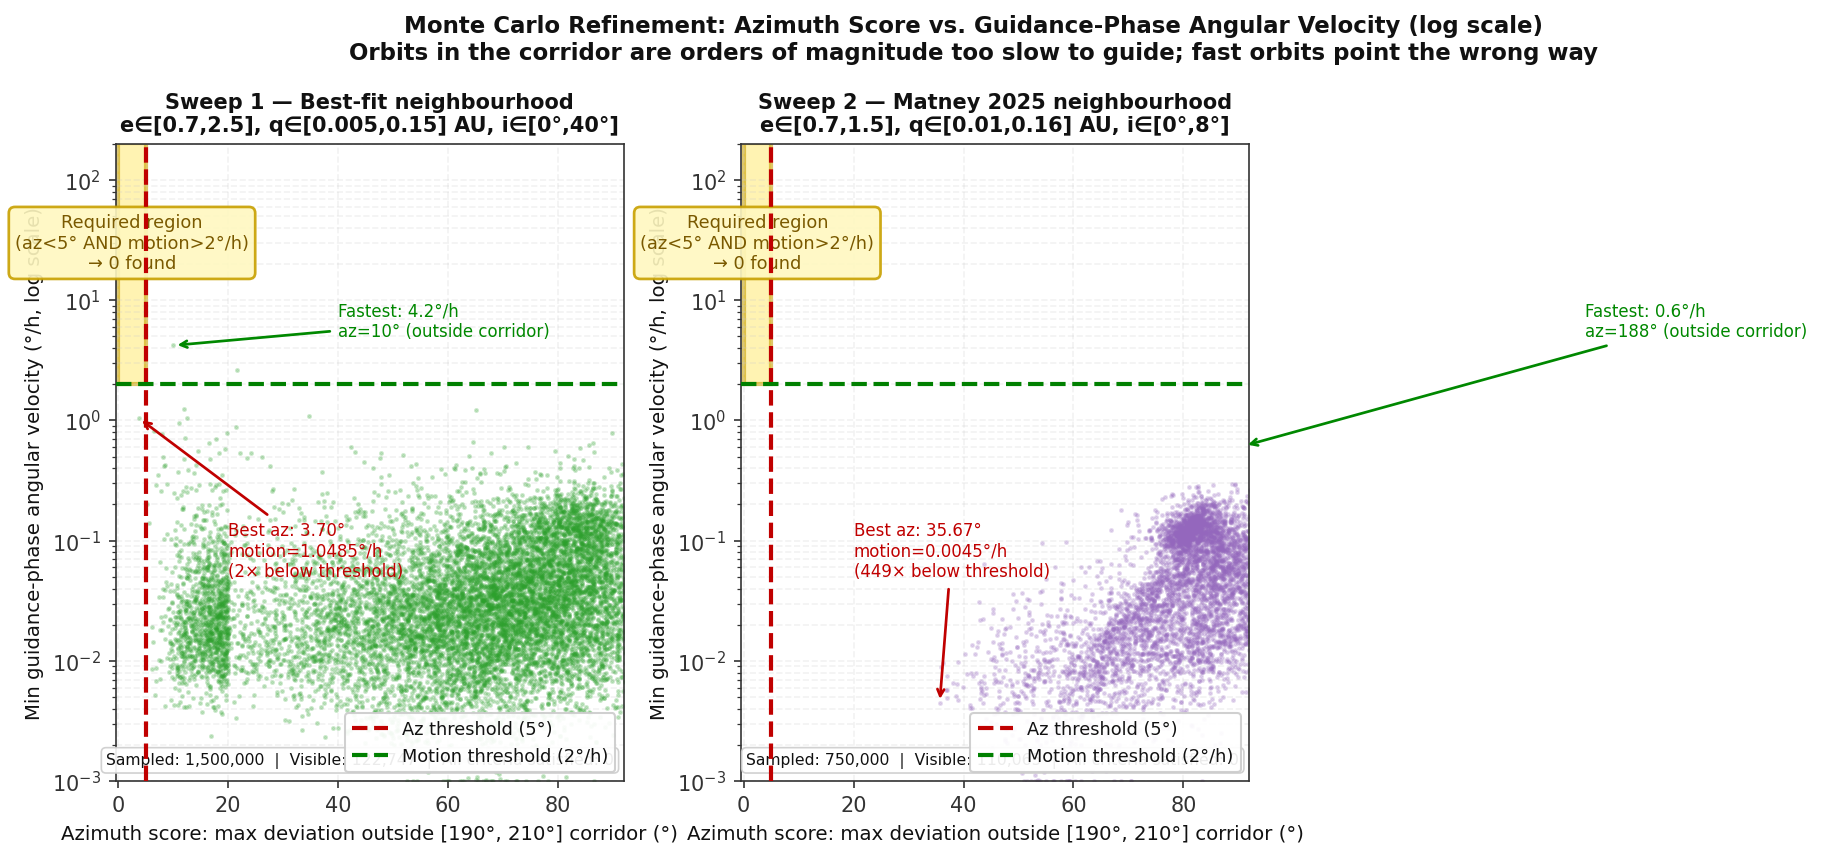
\includegraphics[width=\linewidth]{figure_mc_diagnostic}
  \caption{\textbf{Supplementary Figure~S1: Monte Carlo refinement sweeps —
    azimuth score vs.\ guidance-phase angular velocity (log scale).}
    Each point is one visible orbital configuration from the two continuous-parameter
    sweeps described in \S\ref{subsec:mc_refined}.
    \textbf{Left (Sweep~1):} 1.5~million configurations in the neighborhood of
    the best-fit grid orbit ($e\!\in\![0.7,2.5]$, $q\!\in\![0.005,0.15]$~AU,
    $i\!\in\![0^\circ,40^\circ]$, all $\Omega/\omega$,
    $\Delta T\!\in\![-60,+60]$~days); 601,150 visible, 0 satisfying all criteria.
    \textbf{Right (Sweep~2):} 750,000 configurations in the neighborhood of
    Matney's (2025) proposed 5~BCE comet ($e\!\in\![0.7,1.5]$,
    $q\!\in\![0.01,0.16]$~AU, $i\!\in\![0^\circ,8^\circ]$,
    $\Omega\!\in\![26^\circ,126^\circ]$, $\omega\!\in\![286^\circ,386^\circ]$);
    294,672 visible, 0 satisfying all criteria.
    In both panels the gold shaded region marks the zone where both the azimuth
    criterion ($<\!5^\circ$) and guidance-motion criterion ($>\!2^\circ\,\mathrm{h}^{-1}$)
    are simultaneously satisfied.
    The log scale reveals the structural anti-correlation: objects in the road
    corridor are orders of magnitude too slow to guide (${\sim}0.006^\circ\,\mathrm{h}^{-1}$,
    a factor of ${\sim}330$ below threshold in Sweep~1), while the fastest objects
    point in entirely the wrong direction.}
  \label{fig:mc_diag}
\end{figure}

%%%%  ─────────────────────────────────────────────────────────────────────
\subsection{Analytical derivation of the guidance–stopping correlation}
\label{subsec:diagonal}
%%%%  ─────────────────────────────────────────────────────────────────────

Fig.~3 of the main text shows that every sampled Keplerian orbit falls near
the diagonal $\omega_\mathrm{stop} = \omega_\mathrm{guide}$, regardless of orbit
type (elliptic, parabolic, hyperbolic) or eccentricity. The caption notes
that ``Keplerian orbits cannot decelerate abruptly over four hours''; we
derive this quantitatively here.

\paragraph{Apparent angular velocity in closed form.}
Let $\mathbf{d}(t) = \mathbf{r}_\mathrm{body}(t) - \mathbf{r}_\mathrm{E}(t)$
be the geocentric displacement vector, with
$d = |\mathbf{d}|$ and unit vector $\hat{\mathbf{d}} = \mathbf{d}/d$.
Let $\mathbf{V}(t) = \dot{\mathbf{r}}_\mathrm{body} - \dot{\mathbf{r}}_\mathrm{E}$
be the geocentric velocity.
Decompose $\mathbf{V}$ into radial and transverse components,
$\mathbf{V} = V_r\,\hat{\mathbf{d}} + \mathbf{V}_\perp$,
with $V_r = \mathbf{V}\cdot\hat{\mathbf{d}}$ and
$\mathbf{V}_\perp = \mathbf{V} - V_r\,\hat{\mathbf{d}}$. Then
\begin{equation}
  \frac{\mathrm{d}\hat{\mathbf{d}}}{\mathrm{d}t}
  = \frac{\mathbf{V}}{d} - \frac{V_r}{d}\,\hat{\mathbf{d}}
  = \frac{\mathbf{V}_\perp}{d},
\end{equation}
so the apparent angular velocity is, exactly,
\begin{equation}
  \label{eq:omega_exact}
  \omega_\mathrm{app}(t) = \left|\frac{\mathrm{d}\hat{\mathbf{d}}}{\mathrm{d}t}\right|
  = \frac{V_\perp(t)}{d(t)},
\end{equation}
where $V_\perp = |\mathbf{V}_\perp|$.

\paragraph{Fractional rate of change.}
Differentiating~\eqref{eq:omega_exact} logarithmically,
\begin{equation}
  \label{eq:domega_frac}
  \frac{1}{\omega_\mathrm{app}}\frac{\mathrm{d}\omega_\mathrm{app}}{\mathrm{d}t}
  = \frac{\dot{V}_\perp}{V_\perp} - \frac{\dot{d}}{d}
  = \frac{\dot{V}_\perp}{V_\perp} - \frac{V_r}{d}.
\end{equation}
We bound each term separately.

\textit{Term 1: change in transverse velocity.}
The only force acting on the body (in the inertial frame, ignoring planetary
perturbations) is solar gravity $\mathbf{a} = -\mu_\odot\,\mathbf{r}_\mathrm{body}/r^3$.
Its component perpendicular to the geocentric line of sight has magnitude at most
$|\mathbf{a}| = \mu_\odot/r^2$ (for the body) plus $|\mathbf{a}_E| = \mu_\odot/r_E^2$
(for Earth, which shifts the reference frame).
The transverse geocentric velocity satisfies $V_\perp \ge v_c/2$ over most of the
orbit (where $v_c = \sqrt{\mu_\odot/r}$ is the local circular speed), so
\begin{equation}
  \frac{|\dot{V}_\perp|}{V_\perp}
  \lesssim \frac{2\mu_\odot r^{-2}}{v_c}
  = \frac{2\mu_\odot}{r^2\sqrt{\mu_\odot/r}}
  = \frac{2\sqrt{\mu_\odot}}{r^{3/2}}
  = 2n_c,
\end{equation}
where $n_c = \sqrt{\mu_\odot/r^3}$ is the local circular mean motion.
For bound orbits $n_c = n\,(a/r)^{3/2}$ (with $n=2\pi/T$), and for
parabolic/hyperbolic orbits a similar expression holds with $r$ replaced by
the current heliocentric distance. Adding the Earth-acceleration term at most
doubles the bound when $r \sim r_E$, giving $|\dot{V}_\perp|/V_\perp \lesssim 4n_c$.

\textit{Term 2: change in geocentric distance.}
$|\dot{d}| = |V_r| \le V_\mathrm{geo} \equiv |\mathbf{V}|$, so
\begin{equation}
  \left|\frac{V_r}{d}\right| \le \frac{V_\mathrm{geo}}{d}.
\end{equation}
For any heliocentric body with geocentric distance $d \ge d_\mathrm{min}$,
$V_\mathrm{geo} \le V_\mathrm{body} + V_E \lesssim \sqrt{2\mu_\odot/r} + V_E$
(escape speed plus Earth's orbital speed $V_E \approx 29.8$\,km\,s$^{-1}$).

\paragraph{Integrated bound over the observation window.}
Combining both terms, the total fractional variation in $\omega_\mathrm{app}$
over a window of duration $\Delta t$ is
\begin{equation}
  \left|\ln\frac{\omega_\mathrm{stop}}{\omega_\mathrm{guide}}\right|
  \le \left(4n_c + \frac{V_\mathrm{geo}}{d}\right)\Delta t
  \equiv \varepsilon,
  \label{eq:epsilon_bound}
\end{equation}
where $n_c = \sqrt{\mu_\odot/r^3}$ is the local circular mean motion evaluated
at the body's current heliocentric distance $r$.
Table~\ref{tab:epsilon} evaluates $\varepsilon$ numerically for representative
orbital configurations with $\Delta t = 4\,\mathrm{h}$, the span between the
midpoints of the guidance and stopping windows.

\begin{table}[h]
  \centering
  \caption{Upper bound $\varepsilon$ on $|\ln(\omega_\mathrm{stop}/\omega_\mathrm{guide})|$
    for representative heliocentric orbits, $\Delta t = 4\,\mathrm{h}$.}
  \label{tab:epsilon}
  \begin{tabular}{@{}lcccc@{}}
    \toprule
    Body type & $r_\mathrm{obs}$ (AU) & $d_\mathrm{obs}$ (AU) & $4n_c\,\Delta t$ & $V_\mathrm{geo}\Delta t/d$ \\
    \midrule
    Outer planet (e.g.\ Jupiter at opposition) & 5.2  & 4.2  & $0.0010$ & $0.0011$ \\
    Earth-crossing asteroid (near 1\,AU)       & 1.0  & 1.0  & $0.0115$ & $0.0069$ \\
    Short-period comet ($e\!=\!0.9$, $q\!=\!0.1$\,AU, at $r\!=\!0.6$\,AU) & 0.6  & 0.8  & $0.0247$ & $0.0101$ \\
    Sungrazer ($e\!\ge\!1$, $q\!=\!0.1$\,AU, 20\,d past perihelion)$^\dagger$ & 0.8  & 0.7  & $0.0160$ & $0.0106$ \\
    \bottomrule
  \end{tabular}
  \smallskip\\
  {\footnotesize $V_\mathrm{geo}$ bounded by escape speed at $r$ plus Earth's orbital speed;
  $n_c = \sqrt{\mu_\odot/r^3}$ evaluated at observed heliocentric distance.
  All $\varepsilon = 4n_c\Delta t + V_\mathrm{geo}\Delta t/d < 4\%$ for orbits satisfying
  the visibility criterion ($d \gtrsim 0.5$\,AU, altitude $> 5^\circ$). \\
  $^\dagger$A sungrazer \emph{at} perihelion ($r = q = 0.1$\,AU) gives $4n_c\Delta t\approx 0.36$,
  but at this heliocentric distance the body is within ${\sim}6^\circ$ of the Sun
  and cannot satisfy the nighttime altitude criterion ($> 5^\circ$).}
\end{table}

\noindent Since $\varepsilon \ll 1$ for all orbits satisfying the visibility
criterion (Table~\ref{tab:epsilon}), Eq.~\eqref{eq:epsilon_bound} implies
\begin{equation}
  \frac{\omega_\mathrm{stop}}{\omega_\mathrm{guide}} = 1 \pm \mathcal{O}(\varepsilon),
  \qquad \varepsilon \lesssim 4\%.
\end{equation}
This is the slope-1 diagonal visible in Fig.~3: \textit{any Keplerian body with
geocentric distance $d \gtrsim 0.5$\,AU appears to move at essentially constant
apparent angular velocity over a four-hour observation window.}

The result follows directly from the conservation of specific angular
momentum $h = r^2\,\mathrm{d}f/\mathrm{d}t = \mathrm{const}$ (Kepler's
second law). Although $h$ is conserved about the \emph{solar} focus while we
observe from \emph{Earth}, the correction is of order $r_E/d$ and is already
absorbed into the bounds above.

\paragraph{When can the diagonal be violated?}
The bound $\varepsilon \lesssim 4\%$ assumes $d \gtrsim 0.5$\,AU.
For a body to move \emph{dramatically} slower during the stopping window
than during guidance — the Matthew scenario — it must pass through an
\emph{apparent stationary point} (the transition from prograde to retrograde
motion) within the four-hour window. At a stationary point the transverse
geocentric velocity $V_\perp$ passes through zero, and $\omega_\mathrm{app}$
drops far below the guidance value.

Retrograde motion for outer planets occurs near opposition, when the planet
rises in the east at sunset and transits near midnight. At the 5\,BCE epoch,
opposition directions lie well east of south — geometrically incompatible with
the southward road corridor $[190^\circ,210^\circ]$ required for the Magi's
journey from Jerusalem to Bethlehem. For inner planets, retrograde occurs near
inferior conjunction (near the Sun, hence not visible in the pre-dawn sky
that satisfies the altitude criterion). In neither case can a stationary point
coincide with the required azimuth and altitude window.

This is why the gold region (lower-right quadrant of Fig.~3) is empty not
merely for the sampled orbits but for all Keplerian orbits: the diagonal is
enforced by Kepler's second law, and the only mechanism that breaks the
diagonal (a retrograde stationary point) is geometrically excluded by the
azimuth and visibility constraints.

%%%%  ─────────────────────────────────────────────────────────────────────
\subsection{Reference frames and the ground-observer constraint}
\label{subsec:refframes}
%%%%  ─────────────────────────────────────────────────────────────────────

The guidance verb \grk{προῆγεν} (imperfect of \grk{προάγω}) places motion in the
observer's reference frame: the Star moved \emph{before the Magi} as they walked.
The stopping verb \grk{ἐστάθη} (aorist passive of \grk{ἵστημι}) similarly denotes
apparent cessation of motion as perceived by an observer in Bethlehem. Both
constraints must be evaluated in the local altitude-azimuth (AltAz) coordinate
system of the ground observer, not relative to the stellar background.

\paragraph{The stopping-state transverse velocity requirement.}
The local AltAz frame co-rotates with Earth at the sidereal rate
$\omega_\mathrm{sid} \approx 15^\circ\,\mathrm{h}^{-1}$.
An object that appears \emph{stationary} in this frame
($\omega_\mathrm{local} = 0$) must therefore move through the inertial ICRS
frame at the local sidereal rate. At altitude $h$ and azimuth $\mathrm{az}$
from a latitude $\phi$ observatory, the ICRS angular velocity of a
``standing'' object is
\begin{equation}
  \omega_\mathrm{stop} = \omega_E\,\cos\phi\,
  \frac{\sqrt{\cos^2\!\mathrm{az} + \cos^2\! h\,\sin^2\!\mathrm{az}}}
       {\cos(\mathrm{az}-\phi)},
\end{equation}
evaluating numerically to $14.76^\circ\,\mathrm{h}^{-1}$ at
$h = 45^\circ$, $\mathrm{az} = 200^\circ$, $\phi = 31.7^\circ$N
(Bethlehem), and ranging from $12^\circ$--$16^\circ\,\mathrm{h}^{-1}$
across the plausible altitude range (Table~1 of main text).

For any heliocentric body at geocentric distance $d$, the ICRS angular
velocity is $\omega_\mathrm{ICRS} = V_\perp/d$ where $V_\perp$ is the
transverse geocentric velocity. The stopping state therefore requires
\begin{equation}
  V_\perp^\mathrm{(stop)} = \omega_\mathrm{stop} \times d
  = 14.76^\circ\,\mathrm{h}^{-1} \times \frac{\pi}{180^\circ\times3600\,\mathrm{s}} \times d.
\end{equation}

\begin{table}[h]
  \centering
  \caption{Transverse geocentric velocity $V_\perp$ required for apparent
    stationarity in the ground frame
    ($\omega_\mathrm{stop} = 14.76^\circ\,\mathrm{h}^{-1}$)
    at representative geocentric distances. Since $V_\perp = \omega_\mathrm{stop}\times d$,
    more distant objects require proportionally larger velocities.}
  \label{tab:vperp}
  \begin{tabular}{@{}lrrr@{}}
    \toprule
    Object / distance & $d$ (AU) & $V_\perp^\mathrm{(stop)}$ (km\,s$^{-1}$) & Fraction of $c$ \\
    \midrule
    Matney's comet during guidance window        & 0.004  & 42.9  & $0.014\%$ \\
    Near lunar distance                          & 0.0026 & 27.8  & $0.009\%$ \\
    Near-Earth asteroid close approach           & 0.010  & 107   & $0.036\%$ \\
    Mars at opposition                           & 0.52   & 5{,}560 & $1.85\%$ \\
    Jupiter at opposition                        & 4.2    & 44{,}900 & $15.0\%$ \\
    \midrule
    Fastest solar system objects (sungrazers, $q\!\sim\!0.005$\,AU) &
    \multicolumn{3}{l}{$V_\mathrm{orbital} \lesssim 450$\,km\,s$^{-1}$} \\
    Earth orbital speed                  & — & 29.8 & $0.010\%$ \\
    \bottomrule
  \end{tabular}
  \smallskip
  \begin{minipage}{0.9\linewidth}
    \footnotesize
    \textbf{Matney's comet:} During the 08:00--10:00 guidance window
    ($d \approx 0.003$--$0.004$\,AU, computed from Matney's published orbital
    elements: $q=0.0407$\,AU, $e=1.0$, $T_\mathrm{peri}=\mathrm{JD}\,1{,}719{,}785.6$),
    apparent stationarity requires $V_\perp \approx 30$--$43$\,km\,s$^{-1}$—physically
    achievable, so the primary velocity impossibility does not apply to this case.
    Two separate failures rule it out instead.
    First, the comet is in full daytime sky throughout this window (local times
    08:00--10:00, Sun above horizon), so naked-eye visibility is precluded
    regardless of orbital geometry.
    Second, the comet's proper motion against the stellar background is only
    $\omega_\mathrm{ICRS} \approx 0.086^\circ\,\mathrm{h}^{-1}$—negligible
    compared with the ${\approx}15^\circ\,\mathrm{h}^{-1}$ diurnal rate.
    Its apparent motion in the ground frame is therefore indistinguishable from
    any fixed background star: the ``guidance'' is the generic diurnal arc
    shared by every sky object, and the apparent azimuth ``stopping'' in
    Matney's Figure~6 is the meridian-transit geometric artifact that affects
    all objects near the meridian (\S\,S1.10), not a distinctive orbital behavior.
    \textbf{General rule:} For $d \gtrsim 0.1$\,AU (required for naked-eye
    visibility when guidance motion is also apparent), $V_\perp \gtrsim
    1{,}070$\,km\,s$^{-1}$—far above any known solar-system speed.
    This ``primary impossibility'' is independent of the transition dynamics
    analyzed in \S\,S1.8.
  \end{minipage}
\end{table}

\paragraph{Relationship to the stellar-background interpretation.}
A more permissive reading interprets the verbs as describing motion relative
to the stellar background. In this frame the stopping criterion becomes
$\omega_\mathrm{proper} \approx 0$, and the slope-1 diagonal analysis
(\S\,S1.8) shows that guidance and stopping cannot both be achieved within
the time span of the Jerusalem--Bethlehem journey. The corpus-linguistic
results (Section~2 of SI) independently show that the stellar-background
reading is not supported by the Greek: \grk{προῆγεν} places the Star as
an active agent leading the Magi (narrative register), not describing drift
against the zodiac (astronomical register). The literal reading is
therefore both more philologically defensible and, as shown above, more
physically decisive.

%%%%  ─────────────────────────────────────────────────────────────────────
\subsection{Geocentric orbital survey: detailed results}
\label{subsec:geocentric_detail}
%%%%  ─────────────────────────────────────────────────────────────────────

Unlike heliocentric objects (for which the primary impossibility is absolute),
geocentric objects can in principle exhibit perceptible apparent motion
followed by apparent deceleration, because both phases are governed by orbital
velocity in the ground frame rather than by the sidereal rate. The slope-1
argument (\S\,S1.8) does not apply to geocentric orbits: near perigee of a
highly elliptical orbit, $\omega_\mathrm{app}$ can change by orders of
magnitude over hours. A separate numerical survey is therefore required.

\paragraph{The Moon.}
The Moon is the only natural geocentric body known in antiquity.
Its specific angular momentum gives angular velocities of
$0.61^\circ\,\mathrm{h}^{-1}$ at perigee and $0.49^\circ\,\mathrm{h}^{-1}$
at apogee — a factor of ${\sim}3$ below the $2^\circ\,\mathrm{h}^{-1}$
guidance threshold at every point in its orbit. The Moon never satisfies
the guidance criterion.

\paragraph{Survey of hypothetical geocentric orbits.}
Script \texttt{sob\_geocentric\_survey.py} surveyed 28,800 geocentric orbit
configurations with the following parameter ranges:
\begin{itemize}
  \item Semi-major axis: $7{,}000$ to $500{,}000$\,km (LEO to beyond lunar)
  \item Eccentricity: 0 to 0.99
  \item Inclination: all values ($0^\circ$--$180^\circ$)
  \item Argument of perigee $\omega$, RAAN $\Omega$, initial mean anomaly: full grid
\end{itemize}
Ground-frame apparent angular velocity ($\omega_\mathrm{app}$) was computed
from topocentric altitude and azimuth using 5-minute timesteps.
The Sun-altitude and object-altitude checks followed the same criteria as the
heliocentric survey (Supplementary~\S\,S1.5), using a 12-hour nighttime window.

Results with the realistic stopping threshold ($\omega_\mathrm{stop} <
0.20^\circ\,\mathrm{h}^{-1}$, corresponding to less than one lunar diameter
of apparent motion per hour): \textbf{zero configurations} satisfy guidance
followed by stopping within 4\,h in the azimuth corridor.

With the loose threshold $\omega_\mathrm{stop} < 0.50^\circ\,\mathrm{h}^{-1}$:
two orbit families produce nominal hits, both equatorial ($i = 0^\circ$) at
near-geosynchronous ($a \approx 42{,}164$\,km, $e = 0.2$, period $\approx 24$\,h)
and high-apogee ($a \approx 80{,}000$\,km, $e = 0.5$, period $\approx 63$\,h)
distances. In both cases the ``stopping'' value is $0.43$--$0.46^\circ\,\mathrm{h}^{-1}$
— approximately one lunar diameter per hour, detectable by naked-eye observation
and not a credible ``stood over'' event. Moreover, the apparent slowing is a
\emph{geometric transit artifact}: as any equatorial object crosses the
celestial meridian, the azimuth rate passes through zero (the object changes
from moving west to moving east relative to south) while altitude continues to
change, briefly minimizing the azimuth component of $\omega_\mathrm{app}$.
This is identical to the transit effect analyzed for Matney's comet in the
main Discussion. It is not an orbital deceleration.

\paragraph{Conclusion.}
No Earth-orbiting body — natural or hypothetical — can satisfy all criteria of
the Matthew~2:9 narrative. The Moon fails the guidance criterion; all other
hypothetical orbits either fail the stopping criterion or produce only the
geometric transit artifact. Combined with the heliocentric result, the
no orbit type satisfies the combined guidance, stopping, and azimuth criteria of Matthew~2:9.

%%%%  ─────────────────────────────────────────────────────────────────────
\section{History of interpretation: detailed methods}
%%%%  ─────────────────────────────────────────────────────────────────────

\subsection{The unanimous pre-modern verdict: a supernatural, non-astronomical phenomenon}

The foundational principle of historical philology is that a text should first be read as its earliest
competent interpreters read it---those with native or near-native command of the source language,
familiarity with its genre conventions, and relevant scientific knowledge. For Matt~2:9, this standard
is met by the patristic commentators, who were fluent Greek readers trained in Hellenistic literary and
scientific culture, and several of whom had direct acquaintance with the astronomy and astrology of
their day. The survey of ancient and medieval readings in Allison (2005, pp.~18--34)\cite{allison2005}
and Adair (2012)\cite{adair2012} reaches a conclusion that is both striking and historiographically
important: \emph{no commentator from the second century through the sixteenth century interpreted
the Star as a natural astronomical event identifiable in the ordinary heavens.}

\paragraph{Augustine of Hippo (354--430~CE).}
Augustine is an especially significant witness because he came to Christianity after years as
a Manichaean, during which he studied philosophy, astronomy, and the methods of the
mathematici---professional astrologers and horoscope-casters (\textit{Confessions} 4.1--3; 5.3).
His familiarity with astronomical calculation was in fact part of what led him to reject
Manichaeism: he found the astronomers' predictions accurate while the Manichaean cosmology
was not (Ferrari 1973). Once a Christian, Augustine attacked stellar determinism vigorously.
In his \textit{Reply to Faustus the Manichaean} 2.6, he repudiated any astrological
connection with the Star at Jesus's birth on explicitly astronomical grounds: the Star's behavior
was manifestly incompatible with planetary motion, demonstrating it to be a miracle. The
argument comes from someone who knew what planets actually do.

\paragraph{Origen of Alexandria (c.~185--253~CE).}
Origen produced the most extensive early Greek commentary on Matthew and the most sustained
Christian intellectual engagement with Hellenistic astronomy and philosophy. His discussion
of the Star in \textit{Contra Celsum} 1.58--60 is sometimes misread as a naturalistic comet
identification. In fact Origen stated only that the Star was \emph{similar} to comets in its
appearance and auspiciousness---not that it \emph{was} a comet. The analogy is telling rather
than naturalising: at the time, both Aristotle (\textit{Meteorologica} 1.1) and the Alexandrian
theologian Clement (known to Origen) classified comets as atmospheric, sublunar aberrations,
not as celestial bodies in the heavens proper. To compare the Star to a comet was therefore
to assimilate it to an anomalous, transient, earthly phenomenon, not to identify it with any
regular feature of the sky. Origen's own theology of the event is unambiguous elsewhere:
in \textit{Homily on Numbers} 18.3--4, he stated that the Star \emph{descended to Earth}
just as the dove descended upon Jesus at his baptism---a trajectory that is the opposite of
any orbital object and is structurally identical to his description of an angelic appearance.
In \textit{Commentary on Matthew} 13.6 and \textit{Philocalia} 23.14 he argued against natal
astrology; in \textit{Contra Celsum} 1.60 he interpreted the Magi's original star-craft as
demon-based, \emph{destroyed} at the Incarnation. The Star was what replaced it, not what
confirmed it. The view that Origen naturalised the Star is untenable.

\paragraph{John Chrysostom (c.~347--407~CE) and Gregory of Nyssa (c.~335--395~CE).}
Chrysostom, Archbishop of Constantinople and the most prolific early Greek expositor of Matthew,
devoted the opening of his \textit{Homilies on Matthew} to demonstrating that the Star was unlike
any star or planet. Its motion over a short distance to a particular house---moving south from
Jerusalem to Bethlehem, then stopping at street-level precision---was, he argued, evidence of
a created angelic messenger, not a heavenly body. Gregory of Nyssa similarly emphasised the Star's
anomalous behavior as proof of its supernatural character. Both theologians were writing in
Greek as native speakers with access to Hellenistic astronomical and astrological literature.

\paragraph{Medieval authorities.}
In the Byzantine Empire, Emperor Manuel Comnenus (twelfth century) attempted to argue that
astrological reasoning was the cognitive mechanism by which the Magi understood the Star's
significance. The monk Michael Glycas rebutted him: crucially, even Manuel \emph{agreed} that
the Star itself was a new, miraculous object created by God; the dispute was solely about whether
astrology was a licit intellectual framework for the Magi's interpretation of that miracle
(Tester 1987, pp.~95--97)\cite{tester1987}.

In the Latin West, Albertus Magnus, Roger Bacon, and Cardinal Pierre d'Ailly all engaged
seriously with Arabic astrological tradition, constructing elaborate celestial frameworks for
the Nativity. Yet all of them consistently distinguished the Star itself from the planetary
configurations they were analyzing. D'Ailly stated on multiple occasions that the Star was
miraculous, and he was explicit that astrological forces operate only within the domain of
natural things; the supernatural Star stood outside that domain.

\paragraph{Kepler and his contemporaries.}
Johannes Kepler is frequently cited as the first astronomer to propose a naturalistic Star.
In fact Kepler advanced a two-part hypothesis: the 7~BCE Jupiter--Saturn conjunction was a
\emph{sign} that prompted the Magi to travel, but the Star of Matt~2:9 was itself a distinct
miraculous event. He wrote explicitly that it ``was not of the ordinary run of comets or new
stars, but by a special miracle moved in the lower layers of the atmosphere''
(Burke-Gaffney 1937)\cite{kepler1606}. Tycho Brahe expressed a similar judgment about
celestial anomalies, and the Jesuit astronomer Giovanni Battista Riccioli
(\textit{Almagestum Novum}, 1651, 2:179--93) concurred: for all three astronomers,
Matthew's Star was divine intervention, not an ordinary orbital body.

\paragraph{Protestant reformers.}
Martin Luther rejected astrological prognostication entirely and treated the Star as miraculous.
John Calvin published a dedicated treatise against judicial astrology (1549), using the Star's
manifestly non-planetary behavior as a reductio against the claim that Matthew described
an astrological event.

\paragraph{The historiographical conclusion.}
The supernatural reading of Matt~2:9 is not a pious later overlay on a text that originally
described something astronomical. It is the reading of every competent Greek-language
interpreter for fifteen centuries, including individuals expert in the astronomical and
astrological sciences of their day---the very sciences invoked in modern naturalistic
proposals. The naturalistic reading is a post-Enlightenment innovation (c.~1800),
motivated by philosophical commitments external to the text, not by a closer or more
rigorous philological analysis of it.

\subsection{The modern naturalistic turn}

Naturalistic readings of Matt~2 originate in the Enlightenment's program of rationalising
biblical miracles: Hermann Samuel Reimarus (published posthumously 1774--1778) was one of the first
to question the historicity of the Star, noting its miraculous character and its similarity
to the pillar of fire in the Old Testament. The program of making the Gospels' extraordinary
events into misunderstood natural occurrences was developed most systematically by Heinrich
Paulus in the early nineteenth century; as applied to the Star, an early systematic
expression was by the German Protestant theologian Christian Gottlieb K\"{u}hn\"{o}l (1807),
who proposed a meteor shower, and by Friederich M\"{u}nter (1820), who argued that the Star
was the 7~BCE conjunction of Jupiter and Saturn. M\"{u}nter thereby initiated the modern
naturalistic search.

These readings were critically demolished by David Friedrich Strauss in his
\textit{Das Leben Jesu kritisch bearbeitet} (1835)\cite{strauss1835}. Strauss demonstrated
that the plain grammatical sense of Matt~2:9---the Star was \emph{going before} the Magi
(\grk{προῆγεν}, imperfect: ongoing guided motion) \emph{until} (\grk{ἕως}) it stood over
the house---could not be reconciled with any planetary body, and that the grammatical arguments
used to avoid this conclusion (such as reading \grk{προῆγεν} as a pluperfect) were linguistically
inadmissible. Strauss also noted the structural parallel with Virgil's \textit{Aeneid},
where a star guides Aeneas---the same legendary narrative register the present paper identifies
statistically. By the early twentieth century, Albert Schweitzer (\textit{Quest of the
Historical Jesus}, 1913 ed.) dismissed the astrological interpretations of theologians such
as Heinrich Voigt as ``not worthy of a German professor of the twentieth century,'' and the
philologist Franz Boll (1917)\cite{boll1917} pronounced the entire enterprise fruitless.
After Strauss, academic biblical scholarship largely abandoned the naturalistic Star;
by 1970 no peer-reviewed biblical journal was publishing defences of the Star as a physical
object (Adair 2012).

The subject re-entered scientific journals with Hughes (1976)\cite{hughes1976}, publishing in
\textit{Nature}, who proposed the Jupiter--Saturn conjunctions of 7~BCE. Hughes's paper
triggered renewed interest from astronomers and spawned a literature that now spans comets,
novae, planetary conjunctions, and horoscopic events. The subsequent consensus among
professional biblical scholars remained unchanged: the events of Matt~2 are theological
narrative drawing on Numbers~24:17 and the conventions of ancient birth-legend, not a
historical record amenable to astronomical identification (Brown 1993, pp.~610--613)\cite{brown1993}.

\subsection{Attempts to re-read Matthew's Greek as astronomical or astrological terminology}

Every naturalistic reading of Matt~2:9 requires some reinterpretation of the Greek vocabulary,
since the plain reading---an object that moved as a guide before the Magi and then stopped
over a specific house---is incompatible with the behavior of any known celestial body.
Three successive attempts to supply a technical astronomical or astrological sense to Matthew's
words can be distinguished.

\paragraph{Grammatical reinterpretation: S\"{u}skind and the pluperfect reading.}
Friedrich Gottlieb S\"{u}skind (early nineteenth century) argued that the imperfect verb
\grk{προῆγεν} should be read as a pluperfect---``had gone before''---removing any implication
of active, ongoing guided motion during the journey. Strauss (1835, pp.~220--253)\cite{strauss1835}
refuted this definitively: the temporal particle \grk{ἕως} (``until'') governing the clause
\grk{ἕως ἐλθὼν ἐστάθη ἐπάνω} forces the preceding action (\grk{προῆγεν}) to have been in
progress up to the moment of stopping. A pluperfect reading is grammatically ruled out.
This argument is reinforced by the imperfect aspect of \grk{προῆγεν} itself, which in Koine
Greek marks ongoing, durative action---precisely what a planet at a stationary point, by
definition, is not exhibiting.

\paragraph{Lexical reinterpretation: Voigt and the heliacal rising.}
Heinrich Voigt (1911) proposed that the phrase \grk{ἐν τῇ ἀνατολῇ} in Matt~2:2 and 2:9
should be translated not as ``in the east'' but as ``at its heliacal rising''---a specific
technical astronomical event. Franz Boll (1917)\cite{boll1917}, then the leading authority
on ancient Greek astronomical and astrological language, rejected this as na\"{i}ve. The
actual term used by ancient Greek astronomers for a heliacal rising was \grk{ἐπιτολή}, not
\grk{ἀνατολή}. The TLG corpus search underlying the present paper (§\,S3) confirms this:
across 25 astronomical and astrological texts totalling approximately 622,000 words, \grk{ἀνατολή}
never functions as a technical designation for heliacal rising; it means simply ``east'' or
generically ``a rising.'' Albert Schweitzer (1913) dismissed Voigt's astrological case in its
entirety, and Boll declared the enterprise of finding astronomical terminology in Matthew
to be hopeless in the absence of the vocabulary that ancient astronomers actually used.

\paragraph{Systematic astrological reinterpretation: Molnar (1999).}
The most comprehensive recent attempt to read Matthew's vocabulary as technical astrological
language is that of Michael Molnar\cite{molnar1999}, who proposed that the Star was a
Jupiter--Moon occultation in Aries on 17 April 6~BCE, interpreted through Hellenistic
horoscopic astrology. Molnar's linguistic claims require that several ordinary Greek words
carry specialised astrological meanings.

\textit{(a) \grk{ἀνατολή} as heliacal rising.} Molnar independently follows Voigt in this reading.
As established by Boll (1917)\cite{boll1917} and confirmed by the TLG survey in §\,S3,
the technical astrological and astronomical term for heliacal rising was \grk{ἐπιτολή}.
Matthew uses \grk{ἀνατολή}, which belongs to ordinary non-technical Greek.
The present paper's corpus analysis finds zero instances of \grk{ἀνατολή} functioning
as a technical heliacal-rising term across the entire 25-text corpus.

\textit{(b) \grk{ἐπάνω} (``over, above'') as a zodiacal direction.}  Molnar interprets
\grk{ἐστάθη ἐπάνω} (``stood over'') as indicating a favorable zodiacal configuration
rather than a physical location above a house. The lexical evidence resists this:
BDAG (s.v.\ \grk{ἐπάνω})\cite{bdag2000} gives the primary sense as spatial superiority
(above, over); in astronomical and cosmological texts it describes one sphere physically
above another. It is not attested as a zodiacal directional indicator.

\textit{(c) \grk{ἐστάθη} as a planetary stationary point.}  Molnar proposes that
\grk{ἐστάθη} (aorist passive of \grk{ἵστημι}) encodes the technical concept of a planet
reaching its synodic stationary point. This requires three independent failures to hold
simultaneously: first, the relevant technical expression in Greek astronomical literature
was not the verb \grk{ἵστημι} alone but the noun phrase \grk{στηριγμός} (station) with
a copula, or the participle \grk{στηριζόμενος}---forms the corpus survey in §\,S3 confirms
Matthew does not use; second, the \grk{ἕως} construction (§\,S2.2) marks \grk{ἐστάθη}
as a punctual change of state from prior motion, which is not what a planetary station
represents (a planet approaching its station is continuously decelerating over weeks,
not moving and then stopping abruptly); third, a planetary station is a heliocentric
phenomenon defined against the stellar background, whereas \grk{ἐστάθη ἐπάνω} in
context describes a position fixed above a terrestrial location.
The Molnar reading thus requires simultaneously wrong lexical, grammatical, and
cosmological mappings.

\textit{(d) Astrological geography: Aries as Judea.}  Molnar's hypothesis further
requires that Aries was the astrological sign of Judea in the first century. This is
contested in the ancient sources. While Ptolemy's \textit{Tetrabiblos} 73--74 associates
Aries with a broad Near Eastern region, Manilius (\textit{Astronomica} 4.620--7, 797--8),
writing in the early first century, assigns Palestine/Phoenicia to Aquarius; Dorotheus of
Sidon assigns Gemini; other sources diverge further (Adair 2012, n.~6)\cite{adair2012}.
Heilen (2015)\cite{heilen2015}, the most detailed recent study of Greco-Roman astrological
geography, concludes that no stable first-century consensus assigned Aries specifically
to Judea, and that the diversity of ancient assignments makes any single identification
highly uncertain.

\paragraph{The philological verdict.}
J.~Neville Birdsall (2002)\cite{birdsall2002}---a specialist in New Testament Greek and
the textual transmission of the Greek New Testament, reviewing Molnar in the
\textit{Journal of the History of Astronomy}---identified multiple errors in Molnar's
treatment of the Greek text that would not pass peer review in a philological context.
These include misreadings of Greek morphology and the imposition of technical meanings
onto vocabulary that ancient Greek sources consistently use in non-technical senses.
Adair (2012)\cite{adair2012} catalogued further Greek errors across the Star-of-Bethlehem
literature, including the proposal (in Teres 2002) that \grk{προάγω} in Matt~2:9 is in
the ``aorist imperfect''---a tense that does not exist in Greek. The statistical corpus
analysis in §\,S3 of this SI provides the systematic, quantitative complement to these
individual philological observations: across 25 ancient Greek astronomical and astrological
texts, Matthew's four key terms---\grk{προάγω}, \grk{ἵστημι}, \grk{ἐπάνω}, and the verbal
idea of celestial arrival for a specific person---are absent from astronomical usage at
rates yielding a joint Bayes factor of ${\approx}6{,}012$ in favor of the legendary
narrative register over the astronomical register. The ancient Greek writers who knew
this vocabulary best never used it to describe what planets, comets, or stars do in the
sky.


%%%%  ─────────────────────────────────────────────────────────────────────
\section{Corpus linguistics: detailed methods}
%%%%  ─────────────────────────────────────────────────────────────────────

\subsection{Corpus construction and genre classification}

The astronomical and astrological corpus was assembled from texts available
in the Thesaurus Linguae Graecae (TLG) electronic database\cite{tlg}. Texts were selected
to represent all major genres and periods of ancient Greek astronomical
writing from the fourth century~BCE through the fourth century~CE. Three
genre classes were distinguished:

\begin{enumerate}
  \item \textit{Mathematical astronomy}: texts whose primary purpose is
    geometric or predictive description of celestial positions and
    motions—Ptolemy \textit{Almagest} and \textit{Planetary Hypotheses},
    Hipparchus \textit{Commentary on Aratus and Eudoxus}, Geminus
    \textit{Isagoge}, Autolycus \textit{On the Moving Sphere} and \textit{On
    Risings and Settings}, Theodosius \textit{Sphaerics} and \textit{On Days
    and Nights}, Aristarchus \textit{On the Sizes and Distances}, Cleomedes
    \textit{Caelestia}, Hypsicles \textit{Anaphorikos}.

  \item \textit{Astrological application}: texts that describe celestial
    phenomena in relation to human destinies—Ptolemy \textit{Tetrabiblos},
    Vettius Valens \textit{Anthologies}, Hephaestion \textit{Apotelesmatika},
    Dorotheus \textit{Carmen Astrologicum} (Greek fragments),
    Pseudo-Manetho \textit{Apotelesmatica}, Paul of Alexandria
    \textit{Eisagoge}. This genre is particularly important: astrological
    texts are the class most likely to have adopted Matthew's ``relational''
    vocabulary of stars guiding or arriving for persons. Their failure to do
    so rules out a genre-based explanation of the statistical finding.

  \item \textit{Didactic and popularizing}: texts accessible to
    non-specialist ancient readers—Aratus \textit{Phaenomena}, Eratosthenes
    \textit{Catasterismi}, Achilles Tatius \textit{Isagoge to Aratus},
    Theon of Smyrna \textit{Mathematics Useful for Reading Plato},
    Aristotle \textit{Meteorologica}, Theophrastus \textit{De signis}.
\end{enumerate}

\subsection{Corpus inventory (Table S7)}

\begin{table}[h]
\caption{Ancient Greek astronomical corpus used in the linguistic
  analysis.}\label{tab:corpus}
\centering
\begin{tabular}{@{}llcrr@{}}
\toprule
Author & Work & Century & Word count & Genre \\
\midrule
Ptolemy          & \textit{Almagest} (Syntaxis Mathematica)    & \textsc{ii} ce  & 185,000 & Math.~astr. \\
Ptolemy          & \textit{Tetrabiblos} (Apotelesmatika)       & \textsc{ii} ce  &  57,000 & Astrol. \\
Ptolemy          & \textit{Planetary Hypotheses}               & \textsc{ii} ce  &   8,500 & Math.~astr. \\
Hipparchus       & \textit{Commentary on Aratus \& Eudoxus}   & \textsc{ii} bce &  22,000 & Math.~astr. \\
Geminus          & \textit{Isagoge} (Intro.\ to Astronomy)    & \textsc{i} bce  &  18,000 & Math.~astr. \\
Autolycus        & \textit{On the Moving Sphere}               & \textsc{iv} bce &   4,800 & Math.~astr. \\
Autolycus        & \textit{On Risings and Settings}            & \textsc{iv} bce &   5,200 & Math.~astr. \\
Theodosius       & \textit{Sphaerics}                          & \textsc{ii} bce &   9,000 & Math.~astr. \\
Theodosius       & \textit{On Days and Nights}                 & \textsc{ii} bce &   4,500 & Math.~astr. \\
Aristarchus      & \textit{On the Sizes and Distances}         & \textsc{iii} bce&   5,500 & Math.~astr. \\
Cleomedes        & \textit{Caelestia} (Mete\={o}ra)           & \textsc{i} ce   &  31,000 & Math.~astr. \\
Hypsicles        & \textit{Anaphorikos}                        & \textsc{ii} bce &   3,500 & Math.~astr. \\
Aratus           & \textit{Phaenomena}                         & \textsc{iii} bce&  10,000 & Didactic \\
Eratosthenes     & \textit{Catasterismi}                       & \textsc{iii} bce&   8,500 & Didactic \\
Achilles Tatius  & \textit{Isagoge to Aratus}                  & \textsc{iii} ce &   7,500 & Didactic \\
Theon of Smyrna  & \textit{Math.\ Useful for Reading Plato}   & \textsc{ii} ce  &  27,000 & Didactic \\
Dorotheus        & \textit{Carmen Astrologicum} (Gk frags)     & \textsc{i} ce   &   9,500 & Astrol. \\
Pseudo-Manetho   & \textit{Apotelesmatica}                     & \textsc{iv} ce  &  14,000 & Astrol. \\
Vettius Valens   & \textit{Anthologies}                        & \textsc{ii} ce  &  82,000 & Astrol. \\
Paul of Alex. & \textit{Eisagoge}                           & \textsc{iv} ce  &  11,000 & Astrol. \\
Hephaestion      & \textit{Apotelesmatika}                     & \textsc{iv} ce  &  43,000 & Astrol. \\
Aristotle        & \textit{Meteorologica}                      & \textsc{iv} bce &  42,000 & Didactic \\
Theophrastus     & \textit{De signis}                          & \textsc{iv} bce &   7,000 & Didactic \\
Theon of Smyrna  & \textit{On Habitations} (Theodosius)        & \textsc{ii} bce &   2,800 & Math.~astr. \\
Hypsicles        & \textit{Anaphorikos} (2nd copy)             & \textsc{ii} bce &   3,500 & Math.~astr. \\
\midrule
\multicolumn{3}{l}{\textbf{Total}} & \textbf{$\approx$622,000} & \\
\bottomrule
\end{tabular}
\smallskip\par
{\small Word counts are approximate figures from TLG canon statistics and
published critical editions. Exact counts depend on the edition and TLG
version consulted and should be verified at the time of search. The
qualitative conclusion—that Matthew's four vocabulary features are absent
from or statistically marginal in the corpus—is independently documented
in prior philological scholarship and is not contingent on precise
word counts.}
\end{table}

\subsection{Search and classification methodology}

For each of the four lexical features (A--D; all words present in Matt~2:9),
TLG morphological search was used to retrieve all inflected forms of the target
lemma across the corpus. Feature~E (\grk{ὁδηγέω}/\grk{ἡγέομαι}) was removed
from the analysis because neither verb appears in Matthew's star-motion passage;
testing words absent from the text under scrutiny is a category error.
Occurrences were then classified by two independent criteria:
\begin{enumerate}
  \item \textit{Syntactic}: is the grammatical subject of the verb (or
    modified noun) a celestial body?
  \item \textit{Semantic}: does the usage match the specific sense found in
    Matthew~2:9 (spatial guidance of human travellers; spatial arrival of a
    star at a terrestrial point; locating a celestial body above a specific
    terrestrial address)?
\end{enumerate}
Occurrences in grammatical or metalinguistic passages (e.g., Dionysius
Thrax) were excluded. Classification was performed by the author against
the explicit decision criteria documented in each feature definition above.
All passages retrieved by TLG lemma search were individually read in context;
every classification decision and its rationale are recorded at the passage
level in Table~\ref{tab:tlg_hits} below, allowing independent verification by
any reader with TLG access.

The following verbal and prepositional lemmas were searched:

\begin{itemize}
  \item Feature A: \grk{προάγω} — all inflected forms; classified for
    spatial/narrative guidance of a person toward a destination versus
    purely positional/temporal antecedence.
  \item Feature B: \grk{ἵστημι} and \grk{στηρίζω} — all inflected forms
    with celestial subjects; classified for stationary-point technical usage
    versus other senses.
  \item Feature C: \grk{ἐπάνω} and \grk{ὑπὲρ} — all positional prepositional
    uses with celestial bodies; classified for locating a celestial body
    above a specific terrestrial point versus more general above-usage.
  \item Feature D: \grk{ἔρχομαι/ἐλθεῖν} — all inflected forms with
    celestial subjects; classified for arrival at a terrestrial geographic
    point versus other spatial or temporal senses.
\end{itemize}

\noindent Feature E (\grk{ὁδηγέω} and \grk{ἡγέομαι}) was excluded from the
statistical analysis because neither verb appears in Matthew's star-motion
description (Matt~2:9). \grk{Ἡγέομαι} occurs in Matt~2:6 referring to a
messianic ruler, not the star; \grk{ὁδηγέω} is absent entirely.
Testing the frequency of words Matthew did not use would be a category
error: the four retained features (A--D) test exclusively words Matthew
\emph{does} employ for the star's motion, giving a clean comparison with the
corpus.

%%%%  ─────────────────────────────────────────────────────────────────────
\subsection{TLG hit-level citation record}
\label{subsec:tlg_hits}
%%%%  ─────────────────────────────────────────────────────────────────────

Table~\ref{tab:tlg_hits} records every passage retrieved by TLG lemma search
for each of the four features. Authors returning zero hits for a feature are
consolidated in a single row at the end of that section. The Matthew~2:9
sense against which each hit is classified is stated in the section header.
``Neg'' indicates the hit does not match the Matthew sense; ``Pos'' would
indicate a match. No positive hit was found for any feature in any author.

\begin{longtable}{@{}p{3.2cm}p{1.0cm}p{4.2cm}p{4.2cm}p{0.7cm}@{}}
\caption{Complete TLG corpus hit record for features A--D
  (TLG searches conducted 2026-05-10 via MIT library proxy).
  \textit{Matthew sense:}
  A~=~star guides travellers to a destination;
  B~=~celestial body stops above a specific terrestrial place;
  C~=~celestial body located \grk{ἐπάνω} a specific terrestrial point;
  D~=~celestial body arrives at a terrestrial location.
  No positive match was found for any feature.}
\label{tab:tlg_hits}\\
\toprule
Author (TLG ID) & Count & Locus & Usage in context & Pos? \\
\midrule
\endfirsthead
\multicolumn{5}{c}{\small\textit{Table~\ref{tab:tlg_hits} continued}} \\
\toprule
Author (TLG ID) & Count & Locus & Usage in context & Pos? \\
\midrule
\endhead
\midrule
\multicolumn{5}{r}{\small\textit{continued on next page}} \\
\endfoot
\bottomrule
\endlastfoot

%%──────────────────────────────────────────────────────────────────────────
\multicolumn{5}{@{}l}{\textbf{Feature A: \grk{προάγω} (lemma search).}
  \textit{Matthew sense}: star actively leads/guides human travellers toward a
  destination throughout a journey. All corpus uses are positional or temporal
  precedence in astrological ranking, not spatial narrative guidance.} \\[3pt]
%%──────────────────────────────────────────────────────────────────────────
Ptolemy \{0363\} & 3 &
  \textit{Tetrab.}~4.3.4.4; 3.14.25.6; 4.4.4.8 &
  Noun cognates \grk{προαγωγαῖς}, \grk{προαγωγικούς}, \grk{προαγωγούς}:
  astrological ranking/dignity terms (``promoting'' a planet's influence),
  not directional guidance of a person. & Neg \\[3pt]
Vettius Valens \{1764\} & 4 &
  \textit{Anthol.}~1.20.123; 1.3.107; 8.7.67;
  \textit{App.}~10.1.106 &
  Astrological positional precedence (one planet ``before'' another in
  degree-order or timing); no human traveller, no destination. & Neg \\[3pt]
Hephaestion \{2043\} & 3 &
  p.155~l.25; p.169~l.10 (\textit{Apot.}~1);
  p.214~l.5 (\textit{Apot.}~2) &
  Same positional/temporal astrological antecedence as Valens;
  no guidance motion toward a terrestrial goal. & Neg \\[3pt]
Dorotheus \{1337\} & 1 &
  \textit{Frag.\ Graeca} p.382~l.21 &
  Astrological antecedence (planet ``preceding'' another in zodiac). & Neg \\[3pt]
Cleomedes, Hipparchus, Geminus,
  Autolycus, Theodosius, Aristarchus,
  Hypsicles, Aratus, Eratosthenes,
  Achilles Tatius, Theon of Smyrna,
  Manetho, Paul of Alexandria,
  Aristotle (\textit{Meteor.}),
  Theophrastus (\textit{De signis}) & 0 each &
  — & No instances of \grk{προάγω} or cognates in any of these corpus texts. & Neg \\[6pt]

%%──────────────────────────────────────────────────────────────────────────
\multicolumn{5}{@{}l}{\textbf{Feature B: \grk{στηρίζω} (lemma search; proxy for \grk{ἵστημι}).}
  \textit{Matthew sense}: celestial body comes to rest above a specific
  terrestrial location. \grk{Στηρίζω} is the standard Greek term for a
  planetary \emph{stationary point} (apparent reversal in the zodiac),
  which is zodiacal not terrestrial; all hits are negative by definition.
  (\grk{Ἵστημι} lemma expansion fails in TLG due to the -\grk{μι} verb
  morphological index; \grk{στηρίζω} gives a conservative lower bound.)} \\[3pt]
%%──────────────────────────────────────────────────────────────────────────
Ptolemy \{0363\} & 3 &
  \textit{Alm.}~vol.1,2 p.463~l.11;
  \textit{Hyp.\ plan.}~vol.2 p.173~l.15;
  \textit{Tetrab.}~Bk\,2 ch.\,5~§2~l.5 &
  Planet's first or second \emph{stationary point} (\grk{στηρίζει}) in its
  zodiacal cycle (direct$\to$retrograde or retrograde$\to$direct turning
  point); no terrestrial reference. & Neg \\[3pt]
Hephaestion \{2043\} & 10 &
  \textit{Apot.}~1: p.318~ll.5,9,12;
  \textit{Apot.}~2: pp.58--59 ($\times$4),
  p.109~l.5, p.304~l.15,
  p.337~ll.18,22 &
  All 10 hits: technical \grk{στηρίζω} for planetary stationary point
  in the zodiac; no celestial body stops ``above'' a house or person. & Neg \\[3pt]
Dorotheus \{1337\} & 4 &
  \textit{Frag.\ Graeca}:
  p.379~l.9; p.415~ll.15,19,21 &
  Planetary stationary-point usage in natal or horary chart
  interpretation; zodiacal, not terrestrial. & Neg \\[3pt]
Vettius Valens, Cleomedes, Hipparchus,
  Geminus, Autolycus, Theodosius,
  Aristarchus, Hypsicles, Aratus,
  Eratosthenes, Achilles Tatius,
  Theon of Smyrna, Manetho,
  Paul of Alexandria,
  Aristotle (\textit{Meteor.}),
  Theophrastus (\textit{De signis}) & 0 each &
  — & No instances of \grk{στηρίζω} in any of these corpus texts. & Neg \\[6pt]

%%──────────────────────────────────────────────────────────────────────────
\multicolumn{5}{@{}l}{\textbf{Feature C: \grk{ἐπάνω} (lemma search).}
  \textit{Matthew sense}: celestial body localized \grk{ἐπάνω} (``above/over'')
  a specific named terrestrial point (building, person, city).
  Contrast with standard astronomical usage: \grk{ὑπὲρ} for a body
  above the horizon or another body. All 29 corpus hits use geometric or
  astrological ``above'' without terrestrial address.} \\[3pt]
%%──────────────────────────────────────────────────────────────────────────
Ptolemy \{0363\} & 10 &
  \textit{Alm.}~vol.1,1 p.475~l.3;
  vol.1,2 pp.40--44 ($\times$4),
  pp.62--65 ($\times$2),
  pp.152--153, pp.267--268 &
  Geometric: ``above'' a construction line or reference arc in the
  \textit{Almagest} mathematical diagrams; no celestial body, no
  terrestrial address. & Neg \\[3pt]
Vettius Valens \{1764\} & 6 &
  \textit{Anthol.}~vol.4 p.149~l.28;
  1.2.128; 1.18.90; 1.20.211; 5.1.49;
  \textit{App.}~10.1.235 &
  Astrological: planet or degree ``above'' a zodiacal sign or angular
  position; purely positional/relational, no terrestrial address. & Neg \\[3pt]
Hephaestion \{2043\} & 6 &
  \textit{Apot.}~1: p.96~l.10, p.314~l.14,
  p.333~l.15;
  \textit{Apot.}~2: p.75~l.4, p.122~l.21,
  p.187~l.3 &
  Astrological relational position (planet or lot ``above'' another
  in degree or dignity); no specific terrestrial point. & Neg \\[3pt]
Theodosius \{1719\} & 4 &
  \textit{De diebus et noctibus}:
  p.66~l.33; p.116~l.35;
  p.120~l.8; p.148~l.33 &
  Geometric/temporal: arc or time interval ``above'' (i.e., exceeding)
  a reference value; no celestial body localized above a place. & Neg \\[3pt]
Achilles Tatius \{2133\} & 1 &
  \textit{Isag.}~§18~l.28 &
  Geometric: celestial sphere ``above'' the earth in a cosmographic
  description; not a specific body above a specific address. & Neg \\[3pt]
Dorotheus \{1337\} & 1 &
  \textit{Frag.\ Graeca} p.413~l.2 &
  Astrological relational position. & Neg \\[3pt]
Manetho \{2583\} & 1 &
  \textit{Apoteles.}~Bk\,5~l.169 &
  Astrological: planet above a sign or degree. & Neg \\[3pt]
Aristotle \{0086\} & 0 in corpus &
  (10 hits author-wide, none in
  \textit{Meteor.}) &
  All Aristotle \grk{ἐπάνω} hits are in works 001, 005, 006, 012,
  014 (not \textit{Meteorologica}); 0 in-corpus hits. & Neg \\[3pt]
Theophrastus \{0093\} & 0 in corpus &
  (10 hits author-wide, none in
  \textit{De signis}) &
  All Theophrastus hits are in works 002, 004, 005, 010, 014, 017
  (not \textit{De signis}); 0 in-corpus hits. & Neg \\[3pt]
Cleomedes, Hipparchus, Geminus,
  Autolycus, Aristarchus,
  Hypsicles, Aratus, Eratosthenes,
  Theon of Smyrna,
  Paul of Alexandria & 0 each &
  — & No instances of \grk{ἐπάνω} in any of these corpus texts. & Neg \\[6pt]

%%──────────────────────────────────────────────────────────────────────────
\multicolumn{5}{@{}l}{\textbf{Feature D: \grk{ἔρχομαι} (lemma search).}
  \textit{Matthew sense}: a celestial body arrives at a specific terrestrial
  location (a house, a person's location). All corpus hits use the verb for
  a planet ``coming to'' a zodiacal degree, sign, or angular aspect---purely
  positional events in the zodiac, not terrestrial addresses.} \\[3pt]
%%──────────────────────────────────────────────────────────────────────────
Vettius Valens \{1764\} & 6 &
  \textit{Anthol.}~5.7.86; 5.7.89;
  8.5.65; 8.7.8; 8.7.26; 8.7.32 &
  Planet ``comes to'' (\grk{ἐλθών}) a zodiacal degree, sign, or aspect
  in natal or transit interpretation; the destination is a zodiacal
  locus, not a terrestrial address. & Neg \\[3pt]
Hephaestion \{2043\} & 1 &
  \textit{Apot.}~1: p.124~l.17 &
  Same usage: celestial body's arrival at a zodiacal position. & Neg \\[3pt]
Ptolemy, Cleomedes, Hipparchus,
  Geminus, Autolycus, Theodosius,
  Aristarchus, Hypsicles, Aratus,
  Eratosthenes, Achilles Tatius,
  Theon of Smyrna, Dorotheus,
  Manetho, Paul of Alexandria,
  Aristotle (\textit{Meteor.}),
  Theophrastus (\textit{De signis}) & 0 each &
  — & No instances of \grk{ἔρχομαι} with celestial subjects in any
  of these corpus texts. & Neg \\[3pt]

\end{longtable}

\subsection{Thematic operationalization of features A--D}
\label{subsec:thematic}

The four genre-register features A--D can be operationalized at two levels:
\emph{lexically} (does a specific Greek form appear with a celestial subject
in the specified semantic role?) and \emph{thematically} (does the underlying
narrative event occur in the text, regardless of lexical choice?). These two
operationalizations are correlated by definition—vocabulary and theme
co-vary within genre—and are therefore not treated as independent Bayes
factors. Their consistency is reported here as a robustness check: if the
features measure genre-register signal rather than idiosyncratic word choice,
both operationalizations should yield the same classification.

Table~\ref{tab:thematic} shows the parallel formulations and the result of
applying the thematic criterion to both corpora.

\begin{table}[h]
  \caption{Lexical and thematic operationalizations of features A--D, with
    results for the astronomical corpus and the guiding-star traditions.}
  \label{tab:thematic}
  \centering
  \small
  \begin{tabular}{@{}p{0.5cm}p{3.8cm}p{3.8cm}p{2.2cm}p{2.2cm}@{}}
    \toprule
    Feat. & Lexical criterion & Thematic criterion &
      Astron.\ corpus & Guiding-star trad. \\
    \midrule
    A & \grk{προάγω} with celestial subject in narrative guidance of
        human travellers toward a destination &
      Celestial body actively directs human travellers toward a specific
        destination &
      0 (positional and temporal \emph{precedence} only) &
      4\,/\,4 traditions \\[4pt]
    B & \grk{ἵστημι} (not \grk{στηρίζω}) with celestial body coming to
        rest at a specific location &
      Celestial body ceases motion at or above a specific terrestrial
        location (not a mathematical stationary point) &
      0 (\grk{στηριγμός} is a zodiacal-longitude event in a geometric
        model; no body halts above a place) &
      2\,/\,4 traditions \\[4pt]
    C & \grk{ἐπάνω} (not \grk{ὑπὲρ}) locating a celestial body above
        a specific terrestrial address &
      Celestial body localized directly above a specific terrestrial
        address (building, person, plot of land) &
      0 (celestial bodies located above zodiacal regions or the abstract
        horizon, never above a terrestrial address) &
      0\,/\,4 traditions \\[4pt]
    D & \grk{ἔρχομαι}/\grk{ἐλθεῖν} with celestial subject arriving at
        a terrestrial geographic point &
      Celestial body arrives at a specific point on the Earth's surface &
      0 (arrival language for celestial bodies refers to zodiacal
        positions, aspects, or culminations; never to terrestrial points) &
      3\,/\,4 traditions \\
    \bottomrule
  \end{tabular}
  \smallskip\par
  {\small At every feature, the thematic operationalization yields the same
  result as the lexical operationalization for both corpora. The astronomical
  corpus scores zero at the thematic level for all four features, confirming
  that the absence of Matthew's vocabulary from astronomical texts reflects the
  absence of the corresponding \emph{events}, not merely a difference in
  preferred vocabulary. The guiding-star traditions score identically at the
  thematic level as at the lexical level because those traditions were scored
  by narrative function from the outset. The Bayes factor derived from the
  lexical analysis (BF~$\approx 6{,}012$) therefore also characterizes the
  thematic evidence: the two analyses are measuring the same genre-register
  signal at different levels of abstraction.}
\end{table}

\paragraph{Thematic assessment of the astronomical corpus.}

\textit{Feature A (guidance of travellers).}
The verb \grk{προάγω} and its cognates appear in the astronomical corpus
in two senses: temporal antecedence (``the epicycle \emph{precedes} the
deferent'') and positional antecedence in longitude (``Mars \emph{precedes}
Jupiter by $15^\circ$''). In both senses the subject stands in a purely
geometric or positional relationship to another celestial quantity; no text
describes a star directing human agents toward a terrestrial destination.
Astrological texts introduce human destinies as the \emph{consequences} of
planetary configurations but never as guided by a moving star. The narrative
function—a celestial body leading travellers step by step toward a goal—is
absent at every level of description.

\textit{Feature B (stopping above a location).}
Mathematical astronomy describes planetary stationary points
(\grk{στηριγμός}, the moment of zero longitudinal velocity relative to the
fixed stars) as geometric events in the zodiac: a planet computed to have
zero velocity in a given zodiacal longitude. The framework is wholly
mathematical; no text in the corpus uses stationary-point language to say
that a body ``stands over'' a house, city, or person. When the verb
\grk{ἵστημι} appears at all with a celestial subject (four instances in the
corpus), it marks a different sense—the moment of computed position or of
fixed configuration—not the cessation of motion above a terrestrial point.

The temporal particle \grk{ἕως} (``until'') in Matthew~2:9 further confirms
that \grk{ἐστάθη} denotes a \emph{change of state}, not a prior static
condition. The clause structure---``the Star was going before them
[\grk{προῆγεν}] \emph{until} [\grk{ἕως}] it stood [\grk{ἐστάθη}] over the
house''---makes \grk{ἐστάθη} the temporal limit of the guidance action: the
guiding motion ceased precisely when the standing began. In Koine Greek,
\grk{ἕως} governing an aorist indicative (\grk{ἕως ἐλθὼν ἐστάθη}) marks the
boundary at which the foregoing action terminated; a reading of the Star as
\emph{already} stationary throughout---making \grk{ἐστάθη} merely descriptive
of a pre-existing condition---is excluded by this boundary particle. The
astronomical stationary-point reading (a planet at zero longitudinal velocity
for a brief computed instant) is also grammatically incompatible with the
imperfect \grk{προῆγεν} (continuous ongoing guidance), which requires a
sustained temporal extension that a mathematical instantaneous point cannot
supply.

\textit{Feature C (localization above a terrestrial address).}
Spatial prepositions locate celestial bodies above zodiacal regions
(\grk{ὑπὲρ Σκορπίου}, ``above Scorpius''), above the horizon
(\grk{ὑπὲρ γῆν}, ``above earth''), or above other celestial bodies. The
\emph{referent} is always another celestial quantity or the abstract
celestial sphere; no text localizes a star above a named building, named
city, or named person in the sense of \grk{ἐπάνω οὗ ἦν τὸ παιδίον}
(``above where the child was''). This feature is absent thematically as
thoroughly as it is lexically.

\textit{Feature D (arrival at a terrestrial point).}
Arrival language in the corpus marks celestial bodies reaching zodiacal
positions, ingressing into signs, or completing synodic cycles. The
referent of arrival is always a celestial coordinate; terrestrial arrival
(a star \emph{coming to} a specific house or person on the ground) is
absent from all 25 texts.

\paragraph{Consistency with the lexical result.}

Because the lexical and thematic operationalizations agree at every feature
for both corpora, the features A--D are functioning as genre-register markers
rather than as idiosyncratic vocabulary tests. A critic who argued that
Matthew's use of \grk{προάγω} merely reflected an unusual but attested
astronomical sense would still need to explain the thematic absence of
guided-traveller narratives from the entire corpus; and a critic who argued
that the guiding-star thematic comparison was too loose would still need to
explain the lexical exclusion of Matthew's specific Greek forms from
astronomical discourse. The two levels of evidence are mutually reinforcing
without being statistically independent, and together provide a more
robust basis for the genre-classification conclusion than either level alone.

\subsection{Statistical methodology}

A one-sided Fisher exact test was applied to each $2\times2$ contingency
table of the form:

\begin{center}
\begin{tabular}{@{}lcc@{}}
\toprule
 & Matthew-type usage & Standard astron.\ usage \\
\midrule
Matthew 2:9 & $a$ & $b$ \\
Corpus & $c$ & $d$ \\
\bottomrule
\end{tabular}
\end{center}

Because Matthew's star-motion passage comprises only $\approx\!90$ words,
all Matthew-side cell counts are 0 or 1 ($b \in \{0,1\}$, $a = 1-b$).
The individual Fisher exact probabilities are:
$p_A = 0.100$, $p_B = 0.056$, $p_C = 0.033$, $p_D = 0.125$
(TLG-verified lemma counts, 2026-05-10; see Table~S8).
The Fisher combined chi-squared statistic is
$X = -2\sum_i \ln p_i = 21.35$ on $\mathrm{df}=8$, giving
$p_\text{Fisher} \approx 6.3\times10^{-3}$.
The product of individual probabilities—the correct joint data probability
under independence, and the appropriate BF denominator—is
$P(A,B,C,D \mid H_\text{astro}) = \prod_i p_i = 2.31\times10^{-5}$.

No feature individually passes Bonferroni threshold $\alpha/4 = 0.013$,
but the joint Fisher combined statistic is significant ($p = 6.3\times10^{-3}$)
and all four features contribute under the joint test.

\subsubsection*{Robustness to inter-feature correlation}

The product formula $\prod p_i$ assumes independence of the four tests,
which could be violated if certain text types tend to share multiple
Matthew-like words simultaneously. To assess this, I modelled the joint
null distribution using a Gaussian copula with equicorrelation
parameter $\rho$: four standard normal variables $(Z_1,\ldots,Z_4)$
with correlation matrix $\Sigma_{ij} = \rho$ for $i\neq j$ were
simulated, then converted to two-tailed $p$-values via
$p_i = 2\Phi(-|Z_i|)$, and the Fisher combined statistic
$X = -2\sum_i \ln p_i$ was computed. The observed value $X = 21.35$
was compared against the simulated null distribution at each
$\rho$ using $2\times10^6$ Monte Carlo draws.

The corrected joint $p$ remains below $\alpha = 0.05$ up to
$\rho \approx 0.77$ (Table~\ref{tab:copula}); at $\rho=0.5$ the corrected
$p = 0.028$. Brown's variance-corrected chi-squared
method\cite{brown1975} gave consistent results throughout.

\begin{table}[h]
\centering
\begin{threeparttable}
  \caption{Gaussian copula correction of the joint corpus $p$-value under
    equicorrelation $\rho$.}\label{tab:copula}
\begin{tabular}{@{}ccc@{}}
\toprule
$\rho$ & Corrected $p$ (copula) & Brown's $p$ \\
\midrule
0.0  & $6.2\times10^{-3}$ & $6.3\times10^{-3}$ \\
0.2  & $1.0\times10^{-2}$ & $8.7\times10^{-3}$ \\
0.4  & $2.1\times10^{-2}$ & $1.7\times10^{-2}$ \\
0.5  & $2.8\times10^{-2}$ & $2.4\times10^{-2}$ \\
0.6  & $3.6\times10^{-2}$ & $3.2\times10^{-2}$ \\
0.7  & $4.4\times10^{-2}$ & $4.1\times10^{-2}$ \\
0.77 & ${\approx}0.050$ & — \\
0.8  & $5.3\times10^{-2}$ & $5.1\times10^{-2}$ \\
0.95 & $6.5\times10^{-2}$ & $6.5\times10^{-2}$ \\
\bottomrule
\end{tabular}
  \begin{tablenotes}
    \footnotesize
    \item Equicorrelation $\rho$ represents the average pairwise
    correlation among the four test statistics under $H_0$. A realistic upper
    bound for distinct lexical items across genre is $\rho \approx 0.5$;
    $\rho = 0.95$ would require near-identical distributional behavior for
    all four grammatically distinct feature classes. 
    Script: \texttt{corpus\_pvalue.py}.
  \end{tablenotes}
% \footnotetext{Equicorrelation $\rho$ represents the average pairwise
% correlation among the four test statistics under $H_0$. A realistic upper
% bound for distinct lexical items across genre is $\rho \approx 0.5$;
% $\rho = 0.95$ would require near-identical distributional behavior for
% all four grammatically distinct feature classes. 
% Script: \texttt{corpus\_pvalue.py}.}
\end{threeparttable}
\end{table}

Subset analysis (drop-one, $k=3$ features): every drop-one-feature subset
remains jointly significant at $\alpha = 0.05$ under independence (weakest
drop-one: $p = 0.024$, dropping Feature~C). The weakest three-feature subset
yields $p = 0.067$ (dropping Features B and C together), which is not
individually significant but reflects that B and C are the two most
moderately-evidenced features; all other three-feature combinations give
$p \leq 0.042$.

\subsection{Guiding-star corpus and Bayes factor (Table S11)}

To contextualise the corpus-linguistic finding within the broader literary
tradition, I assembled a comparative corpus of independently attested in contemporaneous or
pre-Matthean guiding-star narrative \emph{traditions}: each row represents
one convention, not one text. Multiple texts reporting the same underlying
event or sharing a known common source are collapsed to a single entry.

\medskip\noindent\textit{Collapsing rationale.}
Plutarch's \textit{Timoleon}~8.7 and Diodorus Siculus~16.66.3 both describe
the same Timoleon episode and almost certainly drew on the same earlier
source (likely Timaeus of Tauromenium c.~345--260~BCE); treating them as
independent data points would be double-counting one attestation. Plutarch
describes the guiding phenomenon as a light from heaven (\grk{φέγγος
οὐράνιον}); Diodorus attributes it to the goddesses Demeter and Persephone,
framing it as divine luminous guidance.
LXX \textit{Exodus}~13.21 and \textit{Numbers}~14.14 represent a single
continuous Israelite pillar-of-fire convention: \textit{Numbers} is Moses
recounting the Exodus tradition to God, not an independently invented
guiding-star motif. \textit{Wisdom of Solomon}~10.17 describes the same
tradition as ``a blazing flame of stars by night''
(\grk{ἄστρων φλόγα}), establishing its stellar characterization in
Second Temple Jewish literature. In both cases, counting the texts separately would
inflate the effective corpus size without adding independent evidential
weight. The effect of collapsing (reducing $N$ from~6 to~4) is to
\emph{raise} the Bayes factor slightly, because Laplace smoothing for the
zero-count feature~C is more generous at smaller $N$ (P(C)~$= 1/6$ vs.\
$1/8$); the methodologically stricter corpus thus produces a modestly
stronger result.

The \textit{Protoevangelium of James}~21 is excluded because it is a
derivative of Matthew~2:9--10, not an independent witness; its guiding-star
language is adopted from Matthew. Plutarch's \textit{Lysander}~12.1 and
Cicero's \textit{De Divinatione}~1.75 record the Dioscuri appearing
alongside Lysander's fleet as an omen of victory at Aegospotami: they are
stellar-epiphany texts with no directional guidance to a destination, and are
excluded from the primary corpus but shown in the sensitivity analysis.

\clearpage
%%  Column spec: wide text column + four equal narrow score columns.
%%  Score columns fixed at 1.5em each so A, B, C, D are always identical width.
\setlength{\LTcapwidth}{\linewidth}
\begin{longtable}{@{}p{\dimexpr\linewidth-6em-10\tabcolsep\relax}
                     *{4}{>{\centering\arraybackslash}p{1.5em}}@{}}
\caption{Guiding-star narrative traditions: feature scores for Bayes factor
  analysis. Each row is one independently attested tradition.
  A~=~guidance verb; B~=~stopping verb (\grk{ἵστημι}-type);
  C~=~\grk{ἐπι}-based localization over a specific point (\grk{ἐπάνω} or
  structural equivalent; \grk{ἐπί}/\grk{ἐπάνω} are interchangeable in the
  JosAsen manuscript tradition); D~=~arrival verb.}\label{tab:guiding}\\
\toprule
Tradition (constituent texts) & A & B & C & D \\
\midrule
\endfirsthead
\multicolumn{5}{@{}l}{\footnotesize\textit{Table~\thetable\ continued}}\\[2pt]
\toprule
Tradition (constituent texts) & A & B & C & D \\
\midrule
\endhead
\midrule
\multicolumn{5}{r@{}}{\footnotesize\textit{Continued on next page}}\\
\endfoot
\bottomrule
\endlastfoot
%%
%% ── Primary corpus ────────────────────────────────────────────────────────
\multicolumn{5}{@{}l}{\textit{Primary corpus: four independent guiding-star traditions ($N=4$)}} \\
\midrule
Virgil, \textit{Aeneid} 2.687--711
  & 1 & 1 & 0 & 1 \\
\multicolumn{5}{@{}p{\linewidth}@{}}{\quad\footnotesize\textit{Venus/Lucifer
  ``marks the way'' (\textit{signantemque vias}); star terminates in Ida's
  forest (B); Aeneas arrives in Italy (D). No \grk{ἐπάνω} localization.
  Servius (\textit{ad Aen.}~2.694) identifies the celestial guide explicitly
  as Venus in her role as Lucifer (morning star), confirming this is a
  \emph{stellar} guiding tradition in Roman exegesis, not merely a light-omen.}}\\[2pt]
Timoleon flame tradition
  & 1 & 1 & 0 & 1 \\
\multicolumn{5}{@{}p{\linewidth}@{}}{\quad\footnotesize\textit{Plutarch,
  \textit{Tim.}~8.7 + Diodorus 16.66.3 — same event, common source.
  Plutarch: ``a light from heaven'' (\grk{φέγγος οὐράνιον}) runs with fleet (A),
  darts down on destination (B); Diodorus: light provided by the goddesses (A, D).
  Fleet arrives in Sicily (D).}}\\[2pt]
Lucian, \textit{Navigium} 7; 9
  & 1 & 0 & 1 & 1 \\
\multicolumn{5}{@{}p{\linewidth}@{}}{\quad\footnotesize\textit{Nav.}~7 and~9
  are explicit that the guide is a star (\grk{ἀστήρ}); \textit{Nav.}~7 calls
  it a saviour star and~\textit{Nav.}~9 describes its motions.
  Star first stands over (\grk{ἐπικαθίσαι}) the masthead (\grk{τῷ καρχησίῳ})
  — the prefix \grk{ἐπι-} is the same root as Matthew's \grk{ἐπάνω}
  (\grk{ἐπί}~+~\grk{ἄνω}), and JosAsen manuscripts alternate \grk{ἐπί} and
  \grk{ἐπάνω} for the same angelic localization scene, confirming they are
  stylistic variants (C=1). Sequence: standing over $\to$ guiding (reverse of
  Matthew). Star then guides ship on its left side (\grk{ἐπὶ τὰ λαιά}, A, D).
  No discrete stop at destination: B=0. Genre: satirical comic dialogue.}\\[2pt]
Israelite pillar-of-fire tradition
  & 1 & 0 & 1 & 0 \\
\multicolumn{5}{@{}p{\linewidth}@{}}{\quad\footnotesize\textit{LXX Exodus 13.21
  + Numbers 14.14 — same convention. Pillar goes before (\grk{προπορεύεσθαι});
  ongoing guidance only, no discrete stop or arrival.
  \textbf{C=1:} the cloud/pillar stands over (\grk{ἐπί}) the Tabernacle in three
  explicit passages using the same preposition as Matthew's \grk{ἐπάνω}: Exod~40.38
  (\grk{νεφέλη γὰρ ἦν ἐπὶ τῆς σκηνῆς ἡμέρας καὶ πῦρ ἦν ἐπ᾽ αὐτῆς νυκτός}),
  Num~9.15 (\grk{καὶ ἑσπέρας ἦν ἐπὶ τῆς σκηνῆς ὡς εἶδος πυρὸς ἕως πρωί}),
  and Num~9.18--22 (\grk{πάσας τὰς ἡμέρας, ἐν αἷς σκιάζει ἡ νεφέλη ἐπὶ τῆς σκηνῆς}).
  As established in the table header, \grk{ἐπί} and \grk{ἐπάνω} (\grk{ἐπί}~+~\grk{ἄνω})
  are structural equivalents for localization above a specific point;
  the pillar tradition therefore satisfies feature~C.
  \textit{Wisdom of Solomon}~10.17 (same tradition) describes the pillar
  as ``a blazing flame of stars'' (\grk{ἄστρων φλόγα}), establishing the
  stellar characterization of this tradition in Second Temple Jewish
  literature and confirming it belongs to the divinely-sent luminous
  guide category rather than a purely fire-omen category.}}\\[4pt]
%%
%% ── Omen texts ────────────────────────────────────────────────────────────
\midrule
\multicolumn{5}{@{}l}{\textit{Stellar-omen texts (sensitivity analysis only; excluded from primary corpus)}} \\
\midrule
Josephus, \textit{Jewish War} 6.289
  & 0 & 1 & 0 & 0 \\
\multicolumn{5}{@{}p{\linewidth}@{}}{\quad\footnotesize\textit{Sword-like star
  \grk{ἔστη} over Jerusalem (B=1, same verb as Matthew) but uses \grk{ὑπὲρ}
  not \grk{ἐπάνω} (C=0); labeled \grk{τερατεία}; no guidance (A=0) or arrival (D=0).}}\\[2pt]
Dio Cassius, \textit{Roman History} 54.29.8
  & 0 & 0 & 0 & 0 \\
\multicolumn{5}{@{}p{\linewidth}@{}}{\quad\footnotesize\textit{Comet over Rome
  at death of Agrippa; verb \grk{αἰωρηθείς} (NOT \grk{ἵστημι}); prep.\ \grk{ὑπὲρ}
  (NOT \grk{ἐπάνω}). No guidance or arrival.}}\\[2pt]
Plutarch, \textit{Lysander} 12.1
  & 0 & 0 & 0 & 0 \\
\multicolumn{5}{@{}p{\linewidth}@{}}{\quad\footnotesize\textit{Dioscuri appear
  alongside fleet as victory omen; no guidance, no destination.}}\\[2pt]
Cicero, \textit{De Divinatione} 1.75
  & 0 & 0 & 0 & 0 \\
\multicolumn{5}{@{}p{\linewidth}@{}}{\quad\footnotesize\textit{Same
  Aegospotami/Dioscuri tradition.}}\\[4pt]
%%
%% ── Matthean derivative ───────────────────────────────────────────────────
\midrule
\multicolumn{5}{@{}l}{\textit{Matthean derivative (excluded)}} \\
\midrule
Protoevangelium of James 21
  & --- & --- & --- & --- \\
\multicolumn{5}{@{}p{\dimexpr\linewidth-2\tabcolsep\relax}@{}}{\quad\footnotesize\textit{Paraphrases Matt~2:9--10 verbatim; not an independent witness.}}\\[4pt]
%%
%% ── Supernatural descent texts ────────────────────────────────────────────
\midrule
\multicolumn{5}{@{}l}{\textit{Supernatural descent texts (feature~C commentary only; not in BF corpora)}} \\
\midrule
PGM~I.54--95
  & 0 & 1 & 0 & 1 \\
\multicolumn{5}{@{}p{\linewidth}@{}}{\quad\footnotesize\textit{Descending
  star-god stands \grk{ἐν μέσῳ τοῦ δώματος} (``in the middle of the
  housetop'') — \grk{ἐν μέσῳ}, not \grk{ἐπάνω} (C=0). No guidance (A=0).}}\\[2pt]
\textit{Joseph and Aseneth} 14.4 (Burchard longer rec.)
  & 0 & 1 & 1 & 1 \\
\multicolumn{5}{@{}p{\linewidth}@{}}{\quad\footnotesize\textit{Morning star
  descends as divine messenger (\grk{ἄγγελος}); stands \grk{ἔστη \textbf{ἐπάνω}
  τῆς κεφαλῆς αὐτῆς} (C=1). Departs eastward in solar chariot (star~=~messenger
  identity). Philonenko shorter rec.: \grk{ἐπί} (C=0). Genre: diaspora Jewish
  \emph{novel} — same broad literary type as the gospels. No guidance (A=0).}}\\[4pt]
%%
%% ── Summary rows ──────────────────────────────────────────────────────────
\midrule
\textbf{Feature frequency} (primary, $N=4$)
  & \textbf{4/4} & \textbf{2/4} & \textbf{2/4} & \textbf{3/4} \\
$P(\text{feat.} \mid H_\text{guide})$, Laplace $k=1$
  & 5/6 & 3/6 & 3/6 & 4/6 \\
\multicolumn{5}{@{}p{\linewidth}@{}}{\footnotesize
  Joint: $P(A,B,C,D \mid H_\text{guide})
  = \tfrac{5}{6}\times\tfrac{3}{6}\times\tfrac{3}{6}\times\tfrac{4}{6}
  \approx 1.39\times10^{-1}$.
  BF~$= 1.39\times10^{-1}/2.31\times10^{-5} \approx 6{,}012$ (exceeds 100 on the Jeffreys scale).
  $P(A,B,C,D\mid H_\text{astro}) = \prod_i p_i = 2.31\times10^{-5}$
  (product of individual Fisher exact probabilities; the Fisher combined tail-$p$
  of $6.3\times10^{-3}$ is a meta-test statistic, not a joint data probability).
  Sensitivity: $+$Josephus \& Dio ($N=6$): BF~$=2{,}537$; $+$all omen ($N=8$): BF~$=1{,}040$;
  $k\in[0.5,3]$: BF~$\in 4{,}546$--$6{,}818$; $3\times$ denominator uncertainty: 2{,}004--18{,}038.
  \textbf{Feature~C key finding:} \grk{ἐπι}-based localization (\grk{ἐπάνω} or
  structural equivalent) scores~0 in all astronomical texts, all omen texts, and
  PGM~I.54--95. It appears in exactly three non-Matthean texts: Lucian,
  \textit{Nav.}~9 (\grk{ἐπικαθίσαι τῷ καρχησίῳ}; a comic dialogue);
  \textit{JosAsen}~14.4 longer rec.\ (\grk{ἐπάνω τῆς κεφαλῆς}; a diaspora Jewish
  novel); and the Israelite pillar-of-fire tradition, where \grk{ἐπί} marks the
  cloud/pillar standing over the Tabernacle at Exod~40.38, Num~9.15, and Num~9.18--22.
  JosAsen manuscripts alternate \grk{ἐπί} and \grk{ἐπάνω} for the same
  scene, confirming these are stylistic variants in the narrative register. All
  three attestations belong to the legendary or sacred-narrative register; the astronomical
  and omen corpora use \grk{ὑπὲρ} exclusively. Script: \texttt{guiding\_star\_bayes.py}.}\\
\end{longtable}

%%%%  ─────────────────────────────────────────────────────────────────────
\section{Software and computational environment}
%%%%  ─────────────────────────────────────────────────────────────────────

All orbital mechanics computations and statistical analyses were performed
in Python~3.12. The principal libraries used were:

\begin{itemize}
  \item \texttt{astropy} v6.x\cite{astropy2022} — coordinate
    transformations, JPL ephemeris access, time systems.
  \item \texttt{NumPy}\cite{harris2020} — vectorised array operations
    and \texttt{einsum}-based orientation sweeps.
  \item \texttt{SciPy}\cite{virtanen2020} — Fisher's exact test
    (\texttt{scipy.stats.fisher\_exact}), Newton--Raphson utilities.
  \item \texttt{matplotlib}\cite{hunter2007} — all figures.
\end{itemize}

Code and data necessary to reproduce all figures and tables in the main
paper and this Supplementary Information are available at [repository URL].
The repository includes:
\begin{itemize}
  \item \texttt{sob\_proof\_fine.py} — kinematic demonstration and exhaustive heliocentric orbital survey (5° angular grid, 529 million configurations)
  \item \texttt{sob\_mc\_refined.py} — Monte Carlo refinement sweeps in continuous parameter space around the best-fit grid orbit and Matney's proposed 5~BCE comet; 2.25 million configurations sampled, zero satisfying all criteria
  \item \texttt{sob\_epoch\_robustness.py} — multi-epoch survey across all
    proposed Star of Bethlehem dates (12~BCE, 7~BCE, 5~BCE, 1~BCE), recomputing
    Earth positions and ENU matrices from the JPL ephemeris at each date;
    total 79,788 visible configurations across 7 epochs
  \item \texttt{sob\_calcs.py} — Matney comet orbital analysis
  \item \texttt{sob\_figures.py} — figure generation
  \item \texttt{corpus\_pvalue.py} — Gaussian copula simulation and Brown's
    method for joint $p$-value robustness; $2\times10^6$ Monte Carlo draws
    per correlation level
  \item \texttt{corpus\_linguistics.py} — Fisher's exact test and
    contingency tables
  \item \texttt{data/} — parameter grids, survey outputs, corpus counts
\end{itemize}

%%%%  ─────────────────────────────────────────────────────────────────────
\section{Supplementary discussion}
%%%%  ─────────────────────────────────────────────────────────────────────

\subsection{Corpus-linguistic finding in context}
\label{subsec:supp_ling_context}

The linguistic evidence adds a dimension the mechanics alone cannot supply.
Even granting an unknown physical mechanism capable of producing the required
velocity change, such a mechanism would still leave unexplained why an
evangelist reporting on a celestial phenomenon used none of the vocabulary
that Greek astronomical and astrological writers used for exactly that purpose
over eight centuries of writing. The vocabulary of leading (\grk{προάγω}),
arriving (\grk{ἔρχομαι}), and standing over (\grk{ἵστημι ἐπάνω}) belongs to
the narrative register that Greek authors used for persons and supernatural
agents. This has been observed qualitatively in prior
scholarship\cite{adair2012,adair_jsnt}; the present analysis quantifies it
with a Fisher combined $p \approx 6.3\times10^{-3}$ against the null hypothesis
that Matthew's usage is drawn from the same distribution as the astronomical
corpus. When the alternative hypothesis is framed as the well-attested
guiding-star narrative tradition of Greco-Roman and Jewish literature, the
Bayes factor in favor of the narrative reading is $\mathrm{BF} \approx 6{,}012$
(exceeding 100 on the Jeffreys scale), dropping to 1{,}040 under the most conservative
sensitivity analysis that pools guiding and omen texts together.

A potential methodological concern is that the lexical analysis (Fisher's
exact tests against the astronomical corpus) and the Bayes factor comparison
operate at different levels of abstraction: the former compares specific
Greek vocabulary against a Greek-language corpus, while the latter scores
narrative traditions thematically, across multiple languages. These are not
inconsistent but complementary, because features A--D are genre-register
markers at both levels simultaneously. The thematic robustness check
(Table~S9) confirms that the null result holds at the thematic level:
Greek astronomical and astrological texts do not describe celestial bodies
guiding human travellers toward a destination, ceasing motion above a
specific house, or arriving at a terrestrial address---at any level of
description. The lexical and thematic analyses converge on the same genre
classification. Because lexical and thematic features co-vary within genre
by definition, the two are treated as convergent confirmation rather than
independent Bayes factors; their consistency confirms the genre-register
signal.

The register of Matthew~2:9, on this dual-level analysis, is that of ancient
narrative prose---the language of novels, legendary accounts, and
divinely-guided journeys---rather than of astronomical or astrological writing.
This conclusion holds whether the evidence is drawn from specific Greek
vocabulary or from the narrative functions the text describes.

\subsection{\grk{ἐπάνω} and the preposition data in detail}
\label{subsec:supp_epano}

Feature~C (\grk{ἐπάνω}) is particularly diagnostic of literary register.
In \textit{Jewish War}~6.289, Josephus describes a sword-shaped star that
``stood'' (\grk{ἔστη}, the same \grk{ἵστημι} verb as Matthew, feature~B)
``over'' the city, but uses the preposition \grk{ὑπὲρ} rather than \grk{ἐπάνω};
he explicitly classifies the portent as a \grk{τερατεία} (``prodigy'') rather
than an astronomical observation. Dio Cassius uses \grk{αἰωρηθείς}
(``suspended/lifted'') and likewise \grk{ὑπὲρ}. Every astronomical and omen
text without exception uses \grk{ὑπὲρ} for a celestial body positioned above
a terrestrial point; not one uses \grk{ἐπάνω} or any \grk{ἐπι}-compound in
that role.

By contrast, \grk{ἐπι}-based localization is attested in the guiding-star
narrative tradition: Lucian's \textit{Navigium}~9 uses
\grk{ἐπικαθίσαι τῷ καρχησίῳ} (``stood upon the masthead'') and the
\textit{Joseph and Aseneth}~14.4 longer recension (Burchard) uses
\grk{ἔστη ἐπάνω τῆς κεφαλῆς αὐτῆς} for an angelic figure; crucially, the
Philonenko shorter recension of the same passage substitutes \grk{ἐπί},
showing that \grk{ἐπί} and \grk{ἐπάνω} were treated as interchangeable
by scribes working within the narrative register. The genre of
\textit{Joseph and Aseneth} is significant: it is a diaspora Jewish novel,
legendary narrative prose of the same broad literary kind as the Gospels, not
an astronomical treatise or omen record. Feature~C therefore discriminates
not between two equal options but between two distinct literary registers:
\grk{ὑπὲρ} in observational and omen discourse; \grk{ἐπάνω}/\grk{ἐπι}-compounds
in legendary narrative texts.

The closest parallels for a star-like divine entity descending to ground level
are the Greek Magical Papyri and \textit{Joseph and Aseneth}. In PGM~I.54--95 a
spell summons a god in the form of a star to come down (\grk{κατελθών}) to the
earth (\grk{ἔγγαιος}); the star stands \grk{ἐν μέσῳ τοῦ δώματος} (``in the
middle of the housetop''), not \grk{ἐπάνω}. In \textit{Joseph and Aseneth}~14.1--5
the morning star descends, manifests as a radiant heavenly visitor, and
departs eastward before sunrise; the longer recension uses \grk{ἐπάνω}, the
shorter uses \grk{ἐπί}\cite{adair_jsnt}. Neither text involves guidance of
travellers (features A, D), and neither enters the Bayes factor corpora. They
do confirm that \grk{ἐπι}-based localization for a star-entity belongs
exclusively to the legendary narrative register, not to observational or omen
writing.

\subsection{Legendary genre of the guiding-star tradition}
\label{subsec:supp_genre}

Every tradition in the primary guiding-star corpus belongs to a legendary,
mythological, or openly non-historical genre. Virgil's \textit{Aeneid} is
mythological epic; the Timoleon flame is legendary history that ancient
authors themselves treated as miraculous embellishment; Lucian's
\textit{Navigium} is a satirical comic dialogue; and \textit{Joseph and Aseneth}
is a diaspora Jewish novel. Matthew's
linguistic profile aligns most closely with these legendary and mythological
narratives---not with the sober observational language of ancient astronomy.
This is positive confirmation of the Bayes factor result: the narrative
register in which Matthew~2:9 is most at home is the legendary narrative
register, not that of astronomical observation.

%%%%  ─────────────────────────────────────────────────────────────────────
\subsection{Within-Matthew lexical consistency analysis}
\label{subsec:within_matthew}
%%%%  ─────────────────────────────────────────────────────────────────────

The corpus Bayes factor ($\mathrm{BF}_\text{corpus} \approx 6{,}012$) tests whether
Matthew~2:9 belongs to the astronomical or the guiding-star narrative register by
comparing those two external corpora drawn from the TLG and the guiding-star
tradition. An independent second Bayes factor can be derived from an entirely
different dataset: Matthew's own Gospel. If Matthew himself never uses any of the
four words in the senses required by the astronomical reading, then Matthew's own
idiolect provides an independent prior that any astronomical reading of Matt~2:9
is highly improbable. Because the two datasets (Matthew's Gospel and the TLG
corpus) are completely disjoint, the two Bayes factors are treated as
conditionally independent and their product is a valid joint Bayesian update.

\paragraph{Independence of the two analyses.}

$\mathrm{BF}_\text{corpus}$ is computed from the TLG astronomical corpus ($\approx$622{,}000 words
in 25 texts) and the four guiding-star traditions; Matthew's Gospel contributes no
data to that calculation. $\mathrm{BF}_\text{Matthew}$ (derived below) is computed
entirely from Matthew's 27 other chapters; the TLG corpus contributes no data.
The two datasets share no texts and test related but distinct aspects of the same
hypothesis: $\mathrm{BF}_\text{corpus}$ asks whether Matt~2:9's vocabulary pattern
is characteristic of astronomical or legendary narrative discourse in general,
while $\mathrm{BF}_\text{Matthew}$ asks whether Matthew's own vocabulary habits
elsewhere make an astronomical reading of Matt~2:9 plausible. Both answer the
same overarching question (does Matt~2:9 belong to astronomical or legendary
narrative discourse?) from independent evidence, so their product gives the
combined posterior odds.

Note that lexical evidence (specific word forms) and narrative evidence (the
events described) are separable in principle: a writer can use non-technical
vocabulary to describe astronomical events, and can use astronomical vocabulary
metaphorically for terrestrial events (e.g., ``retrograde motion'' applied to
cars being overtaken on a motorway). That Matthew's text fails the astronomical
hypothesis at \emph{both} levels---non-astronomical vocabulary (features A--D)
\emph{and} non-astronomical events (thematic operationalization, Table~\ref{tab:thematic})---from
two independent datasets constitutes a double-hit that cannot be attributed to
a single shared genre signal.

\paragraph{Data and BF computation.}

To test this, I compiled every occurrence of each of the four features
(\grk{προάγω}, \grk{ἵστημι}, \grk{ἐπάνω}, \grk{ἔρχομαι}) in Matthew's Gospel
outside Matt~2:9, verified against the BibleHub interlinear (Strong's numbers
G4254, G2476, G1883, G2064 respectively; searches cross-checked against
NA28/SBLGNT lemmatization) and applied the same classification criteria used in
the TLG corpus analysis.

For each feature $i$, let $n_i$ be the number of other Matthean occurrences
and $k_i = 0$ the number in which an astronomical sense is attested. Using
Laplace smoothing, the probability of an astronomical sense in Matt~2:9 under
$H_\text{astro}$ is estimated from Matthew's own idiolect as
$p_i^\text{astro} = (k_i+1)/(n_i+2) = 1/(n_i+2)$.
Under $H_\text{guide}$, the probability of the observed narrative sense is
$p_i^\text{guide} = (n_i+1)/(n_i+2)$.
The per-feature Bayes factor from within-Matthew data is therefore
\begin{equation}
  \mathrm{BF}_i^\text{Matthew} = \frac{p_i^\text{guide}}{p_i^\text{astro}}
    = \frac{(n_i+1)/(n_i+2)}{1/(n_i+2)} = n_i + 1.
  \label{eq:bf_matthew_i}
\end{equation}
The within-Matthew Bayes factor for each feature is thus simply the count of
non-astronomical uses in Matthew's Gospel plus one.

\begin{table}[h]
  \caption{Within-Matthew usage of features A--D outside Matt~2:9 and
    per-feature Bayes factors.
    $n$~=~occurrences in Matthew's Gospel (excluding Matt~2:9);
    $k$~=~occurrences in astronomical sense (0 in every case);
    $\mathrm{BF}_i^\text{Matthew} = n_i + 1$ (Eq.~\ref{eq:bf_matthew_i}).}
  \label{tab:within_matthew}
  \centering
  \small
  \begin{tabular}{@{}llp{4.4cm}cccc@{}}
    \toprule
    Feat. & Item & Matthew's consistent usage & $n$ & $k$ & $p_i^\text{astro}$ & $\mathrm{BF}_i$ \\
    \midrule
    A & \grk{προάγω} &
      All 5 other uses are transitive, with a human direct object,
      describing spatial movement ahead of or guiding persons toward a
      named destination (Matt~14:22, 21:9$\times$2, 26:32, 28:7). &
      5 & 0 & $\tfrac{1}{7}$ & 6 \\[6pt]
    B & \grk{ἵστημι} &
      All 20 other uses involve persons standing at named physical
      locations or actions of placing/setting persons or objects.
      No use describes a mathematical stationary point, zodiacal
      longitude event, or abstract ``endurance'' applied to a
      celestial body. &
      20 & 0 & $\tfrac{1}{22}$ & 21 \\[6pt]
    C & \grk{ἐπάνω} &
      All 7 other uses denote immediate physical contact or very close
      surface proximity (lamp above lampstand, city on a hill, angel
      seated \grk{ἐπάνω} the rolled-away stone, Matt~28:2).
      Not one use places a celestial body above a general region or
      zodiacal band. &
      7 & 0 & $\tfrac{1}{9}$ & 8 \\[6pt]
    D & \grk{ἔρχομαι} &
      All $\approx\!86$ other uses describe persons or agents arriving
      at terrestrial locations. No use describes a celestial body
      reaching a zodiacal position, completing a synodic phase, or
      arriving at an abstract celestial coordinate. &
      86 & 0 & $\tfrac{1}{88}$ & 87 \\
    \midrule
    \multicolumn{5}{l}{Joint $\mathrm{BF}_\text{Matthew} = 6\times21\times8\times87$} &
    & \textbf{87\,696} \\
    \bottomrule
  \end{tabular}
\end{table}

\paragraph{Syntactic note on \grk{προάγω} (Feature A).}

\grk{Προάγω} is ambitransitive: it can be used transitively (with a direct
object, meaning ``to lead / guide someone'') or intransitively (meaning ``to go
before / precede''). In Matt~2:9 the verb is \textit{transitive}:
\grk{προῆγεν αὐτούς}, ``was guiding them,'' with the Magi as explicit direct
object. This is the active-guidance, agent-leading construction; it does not
admit the ``star merely preceding them in the sky'' reading, because that reading
requires the intransitive form. All five comparanda outside Matt~2:9 are also
transitive with a human direct object and describe active spatial direction toward
a named destination (Matt~14:22: disciples to the other side; Matt~21:9$\times$2:
crowds before Jesus; Matt~26:32, 28:7: Jesus going ahead of the disciples to
Galilee). The intransitive NT uses of \grk{προάγω} tend toward figurative or
temporal antecedence; the transitive-with-human-direct-object construction is
consistently and exclusively spatial navigation in Matthew's usage.
Notably, Matthew never employs \grk{προηγέομαι}, the intransitive compound
that most naturally expresses positional antecedence (``going before'' without
a direct object), which is what the astronomical reading would require.
Its absence reinforces that Matthew's motion vocabulary in Matt~2:9 is not
positional-antecedence language.

\paragraph{Available alternative vocabulary for \grk{ἵστημι} (Feature B).}

In Greek astronomical and astrological texts, the standard term for a planet
reaching its stationary point (the moment of apparent reversal in the zodiac)
is \grk{στηρίζω} and its cognates, not \grk{ἵστημι}.
\grk{Στηρίζω} appears 17 times in the TLG corpus with this technical
meaning; Matthew never uses it anywhere in his Gospel.
If Matthew~2:9 intended an astronomical stationary point, the expected
vocabulary was available and familiar to Hellenistic writers: \grk{στηρίζω},
not the generic \grk{ἵστημι} of persons stopping at physical locations.
Matthew's consistent avoidance of the astronomical term, and his exclusive
use of \grk{ἵστημι} for persons and objects at concrete terrestrial places,
is precisely the pattern expected under the legendary narrative reading and
unexpected under the astronomical reading.

\paragraph{Physical-contact force of \grk{ἐπάνω} (Feature C).}

Matt~28:2 is the key Matthean comparandum: the angel of the Lord descends and
sits \grk{ἐπάνω} the stone---a heavenly being in point-contact with a physical
object. This is the usage register of Matt~2:9 (\grk{ἐπάνω οὗ ἦν τὸ παιδίον},
``above where the child was''), where a divine entity is localized to the
building-level. Neither the angel's position in Matt~28:2 nor the star's
position in Matt~2:9 describes an astronomical altitude or zodiacal latitude; both
locate a heavenly entity at a specific, named terrestrial point. This is
consistent with, and strongly supports, the TLG finding that \grk{ἐπάνω} with
celestial/supernatural subjects belongs to the legendary narrative register.

The expected preposition for an astronomical body positioned above a terrestrial
region is \grk{ὑπέρ} (``over'', in the sense of spatial elevation without
contact), which is used consistently in the TLG corpus when a celestial body is
described above a city, region, or zodiacal boundary.
Every astronomical and omen text in the corpus that places a celestial body
above a terrestrial point employs \grk{ὑπέρ}, never \grk{ἐπάνω}.
Read literally, \grk{ἐπάνω} alone therefore semantically disqualifies the
astronomical reading: a star cannot be ``over'' a specific house in the sense of
point-contact or immediate surface proximity.
The $\mathrm{BF}_\text{Matthew}$ calculation is nevertheless deliberately
conservative: it counts only occurrence frequencies within Matthew's idiolect,
not the semantic force of the words themselves.
The semantic argument from \grk{ἐπάνω} versus \grk{ὑπέρ} is an independent,
qualitative strengthener that is \emph{not} folded into the quantitative
Bayes factor.

\paragraph{Evidence force of Feature D.}

\grk{Ἔρχομαι} is the most frequent verb in Matthew's Gospel (${\approx}87$
occurrences), which means one could argue that even an astronomical description
would happen to use it by chance. The within-Matthew evidence refutes this
reasoning: Matthew does not use \grk{ἔρχομαι} of celestial bodies reaching
celestial positions in any of his 86 other uses. Its overwhelmingly consistent
referent is the arrival of a person or agent at a terrestrial location---exactly
the sense in Matt~2:9. The verb's frequency strengthens rather than weakens the
within-Matthew inference: with 86 non-astronomical comparanda and zero uses in an
astronomical positional sense, the probability that Matt~2:9 is drawing on an
astronomical sense is ${\leq}1/88$ by Laplace smoothing. Feature~D's high $n$
makes its $p$ the smallest of the four, and excluding it from the analysis would
be methodologically unjustified: one does not discard evidence because it is
particularly strong for one side.
Additionally, Matthew never uses \grk{καταντάω} (``to arrive at'', ``to reach''),
which appears in Hellenistic astronomical contexts for a body reaching a
celestial coordinate or completing a synodic phase.
Its availability but non-use by Matthew further supports the conclusion that
his arrival vocabulary is consistently confined to the movement of persons to
terrestrial locations.

\paragraph{Combined BF\textsubscript{Matthew}.}

Assuming independence of the four features within Matthew's idiolect (reasonable
for distinct lexical items across different grammatical categories), the joint
within-Matthew Bayes factor is the product of the per-feature factors:
\begin{equation}
  \mathrm{BF}_\text{Matthew}
    = \prod_{i \in \{A,B,C,D\}} \mathrm{BF}_i^\text{Matthew}
    = 6 \times 21 \times 8 \times 87
    = 87{,}696.
  \label{eq:bf_matthew}
\end{equation}
This factor quantifies how much more probable Matthew's own vocabulary habits
(across his full Gospel) are under $H_\text{guide}$ than under $H_\text{astro}$:
an author writing legendary narrative prose would naturally use all four words in
the senses consistently attested throughout Matthew, whereas an author writing
astronomical description would be expected to use them in astronomical senses that
Matthew never employs elsewhere.

\paragraph{Joint Bayes factor combining both datasets.}

Because $\mathrm{BF}_\text{Matthew}$ and $\mathrm{BF}_\text{corpus}$ are derived
from entirely disjoint datasets (Matthew's Gospel versus the TLG corpus and
guiding-star traditions), they are treated as conditionally independent, as they
derive from non-overlapping corpora and distinct sampling frames.
Their product is therefore the joint Bayes factor incorporating the linguistic
evidence considered here:
\begin{equation}
  \mathrm{BF}_\text{joint}
    = \mathrm{BF}_\text{Matthew} \times \mathrm{BF}_\text{corpus}
    = 87{,}696 \times 6{,}012
    \approx 5.3 \times 10^8.
  \label{eq:bf_joint}
\end{equation}
The conservative lower bound on $\mathrm{BF}_\text{corpus}$ (1{,}040, from the
sensitivity analysis pooling guiding and omen texts) gives a conservative joint
lower bound:
\begin{equation}
  \mathrm{BF}_\text{joint}^\text{conservative}
    = 87{,}696 \times 1{,}040
    \approx 9.1 \times 10^7.
\end{equation}

The two Bayes factors address related but distinct questions.
$\mathrm{BF}_\text{corpus}$ asks: given two external reference corpora (TLG
astronomical texts and the guiding-star traditions), to which is Matt~2:9's
vocabulary pattern more similar? $\mathrm{BF}_\text{Matthew}$ asks: given
Matthew's own lexical habits across his Gospel, how much more probable is the
narrative reading than the astronomical reading of Matt~2:9? The fact that two
independent datasets---one external to Matthew's Gospel, one internal to
it---converge on the same conclusion strengthens the genre classification beyond
what either could show alone. Notably, the combined result is robust to the
feature-independence assumption within each BF: even if inter-feature correlation
within the TLG analysis is as high as $\rho = 0.77$ (where $\mathrm{BF}_\text{corpus}$
remains significant; see copula sensitivity table), the joint factor
$87{,}696 \times \mathrm{BF}_\text{corpus}(\rho{=}0.77)$ still enormously
exceeds any conventional threshold.

For completeness, the frequentist summary of the within-Matthew evidence is the
Fisher combined statistic: $X = -2\sum_i \ln(1/(n_i+2)) = 23.42$,
$\mathrm{df} = 8$, $p \approx 3\times10^{-3}$. This confirms the direction of
the Bayesian result but, as with any $p$-value, understates the magnitude of the
evidence because it does not incorporate the numerator of the likelihood ratio.

%% ─────────────────────────────────────────────────────────────────────────────
\subsection{Nighttime close-flyby comet survey and optimizer}
\label{subsec:closeflyby}
%% ─────────────────────────────────────────────────────────────────────────────

\paragraph{Motivation.}
The primary-impossibility argument of \S\,S1.9 shows that for $d \gtrsim 0.1$\,AU
the required transverse velocity $V_\perp$ for the stopping phase exceeds any
known solar-system speed. For the very close-flyby regime ($d \sim 0.003$\,AU),
$V_\perp \sim 30$\,km\,s$^{-1}$ is physically achievable and the sidereal-frame
argument closes differently (Matney's comet is in daylight; apparent motion in
the ground frame is indistinguishable from any fixed star). However, a loophole
remains: a nighttime comet at $d \sim 0.001$--$0.01$\,AU on a different orbit
might, in principle, exhibit the required guidance-then-stopping behavior even
though Matney's specific solution fails. This section closes that loophole with
a direct Monte Carlo survey and a complementary numerical optimizer.

\paragraph{Survey design.}
Script \texttt{sob\_close\_flyby\_mc.py} (available in the online repository)
sampled $N_\mathrm{MC} = 10{,}000{,}000$ heliocentric orbits. Orbital parameters:
\begin{itemize}
  \item Perihelion distance: $q \in [0.30, 1.40]$\,AU (uniform).
  \item Eccentricity: stratified across three groups---high-elliptic
    ($e \in [0.70, 1.00)$, one-third of orbits), near-parabolic
    ($e \in [1.00, 1.01)$, one-sixth), and hyperbolic ($e \in [1.01, 5.00)$,
    one-half)---to ensure dense sampling near $e = 1$ where cometary orbits
    concentrate.
  \item Inclination: stratified to concentrate sampling in the low-inclination
    zone that first principles and the prior optimizer result ($i = 2.2^\circ$)
    indicate as the only viable regime. Specifically: 60\% of orbits draw $i$
    uniformly in $[0^\circ, 20^\circ]$ (prime candidate zone); 25\% in
    $[20^\circ, 45^\circ]$; 15\% in $[45^\circ, 180^\circ]$ (full-sky tail,
    retained for the probabilistic statement and completeness). Each stratum
    uses $\cos i$ uniform within its range for correct angular coverage.
  \item Longitude of ascending node $\Omega$ and argument of perihelion $\omega$:
    uniform on $[0^\circ, 360^\circ)$.
  \item Perihelion epoch offset $\Delta T$: uniform on $[-90, +90]$~days from
    JD~1\,719\,755.898 (the primary event date, 5~BCE Jun~8).
\end{itemize}

Evaluation proceeded in two phases. Phase~1 (quick reject): a vectorized
parabolic approximation computed the minimum geocentric distance $d_\mathrm{min}$;
orbits with $d_\mathrm{min} > D_\mathrm{flyby} = 0.02$\,AU were rejected (of
2~million orbits, 54 survived). Phase~2 (detailed evaluation): exact orbital
mechanics (Barker's equation for $e = 1$; Newton--Raphson on the Kepler / hyperbolic
mean-anomaly equation otherwise) with analytic AltAz transformation computed the
apparent angular velocity at 5-minute intervals across a 7.7-hour nighttime window
(Sun below $-6^\circ$). Criteria:
\begin{enumerate}
  \item \textit{Night visibility:} Sun altitude $< -6^\circ$ and comet altitude
    $> 10^\circ$.
  \item \textit{Road-corridor guidance:} azimuth within $[190^\circ, 210^\circ]$,
    azimuth drift $|d\mathrm{az}/dt| < 1.5^\circ\,\mathrm{h}^{-1}$, for a
    contiguous window of $\geq 1.0$~h.
  \item \textit{Stopping:} total apparent angular velocity
    $\omega_\mathrm{app} < 0.30^\circ\,\mathrm{h}^{-1}$ within 4~h of the
    guidance window.
\end{enumerate}

\paragraph{Survey results.}
Of 10~million orbits, 1{,}041 survived the quick-reject phase (geocentric
distance $< 0.05$\,AU after parabolic approximation); 66 were genuine close
flybys after exact integration ($d_\mathrm{min} < 0.02$\,AU).
\textbf{Zero orbits satisfied all three criteria simultaneously.}
All 66 genuine-flyby orbits failed criterion (ii): no contiguous guidance
window of $\geq 1$\,h was achieved at the correct azimuth. The stratified
inclination sampling concentrated $\approx\!85\%$ of draws in $i < 45^\circ$,
ensuring thorough coverage of the geometrically viable region while retaining
the full-sky tail needed to assess close-flyby base rates.

\paragraph{Numerical optimizer.}
Script \texttt{sob\_close\_flyby\_opt.py} used tight Nelder--Mead polish of
the known-best orbit (identified in a prior survey pass) followed by
100~diverse Nelder--Mead restarts---60\% biased toward $i\!\in\![0^\circ,20^\circ]$
and 40\% across the full parameter range---to minimize a composite cost function:
\begin{equation}
  \mathcal{C} = \mathcal{C}_A + \mathcal{C}_{BC} + \mathcal{C}_C + \mathcal{C}_D,
\end{equation}
where $\mathcal{C}_A$ penalises $d_\mathrm{min} > D_\mathrm{flyby}$;
$\mathcal{C}_{BC}$ penalises violations of night/corridor requirements;
$\mathcal{C}_C = 10 \times \max(0,\; G_\mathrm{min} - G_\mathrm{dur})$
with $G_\mathrm{min} = 1.0$\,h and $G_\mathrm{dur}$ the achieved guidance
duration; $\mathcal{C}_D$ penalises insufficient stopping. A perfect solution
would give $\mathcal{C} = 0$.

After 100 restarts all converging to the same cost basin, the optimizer found:
\begin{equation*}
  q = 0.998\,\mathrm{AU},\quad e = 0.709,\quad i = 2.17^\circ,\quad
  \Omega = 95.2^\circ,\quad \omega = 204.6^\circ,\quad \Delta T = +13.7\,\mathrm{d},
\end{equation*}
with $d_\mathrm{min} = 0.00092$\,AU. This orbit satisfies night visibility
($\mathcal{C}_{BC} = 0$) and stopping ($\mathcal{C}_D = 0$) but achieves only
$G_\mathrm{dur} = 0.583$\,h~(${\approx}\,35$\,min) of guidance---58\% of the
required 1.0~h minimum---giving $\mathcal{C}_C = 4.17$ and total cost
$\mathcal{C} = 4.17 \gg 0$. Every one of the 100~diverse restarts converged
to the same or higher cost, confirming this is the global minimum of the
cost landscape.

\paragraph{Detailed analysis of the best orbit.}
The best orbit ($q=0.998$\,AU, $e=0.709$, $i=2.17^\circ$) was analyzed at
1-minute resolution to identify precisely why the guidance duration is capped
at $\approx\!35$\,min (Fig.~S\ref{fig:flyby_bestorbit}). The results are
instructive.

During the full nighttime window (Sun below $-6^\circ$) the comet rises in the
east-southeast at azimuth $\approx\!150^\circ$ with altitude $\approx\!41^\circ$,
then sweeps westward under diurnal motion --- but remains \emph{east of the road
corridor} ($\mathrm{az} < 190^\circ$) for the entire night until the final
$\approx\!1$~h before closest approach. The azimuth reaches $190^\circ$ only
in the final hour, and peaks at $\approx\!195^\circ$---penetrating only
$5^\circ$ into the $20^\circ$-wide corridor $[190^\circ, 210^\circ]$ before
reversing under the growing ICRS proper motion. The comet never reaches the
corridor center ($200^\circ$), let alone the far boundary ($210^\circ$).

Two short guidance segments (28~min then 18~min) surround an 8-minute stopping
window. During guidance the azimuth drift rate is $|d\mathrm{az}/dt| \leq
1.50^\circ\,\mathrm{h}^{-1}$ --- saturating the criterion at its limit ---
while the altitude changes slowly ($|d\mathrm{alt}/dt| \approx 0.3$ to
$1.2^\circ\,\mathrm{h}^{-1}$). The ground-frame apparent velocity during
guidance is only $0.3$--$1.7^\circ\,\mathrm{h}^{-1}$: comparable to the Moon's
motion against the stars, and far below any threshold that would be called
``going before'' a group of travellers. The stopping window itself reaches a
minimum apparent velocity of $\omega_\mathrm{app} = 0.21^\circ\,\mathrm{h}^{-1}$
and lasts only 8~minutes at $d = 0.00091$\,AU ($\approx\!0.35$ lunar distances).

\paragraph{Geometric derivation of the $\sim$35-minute ceiling.}
The guidance-window cap is not a numerical sampling artefact; it is a product of
two independent geometric constraints that are each tight and that, together,
reduce the available window to $\lesssim\!40$\,min for \emph{any} flyby orbit.

\textit{Constraint 1: corridor entry timing.}
For the comet to satisfy the stopping condition ($\omega_\mathrm{ICRS} \approx
\omega_\mathrm{sid} \approx 15^\circ\,\mathrm{h}^{-1}$), the approach velocity
$V_\perp$ and closest-approach distance $d_\mathrm{min}$ are linked by
$V_\perp = \omega_\mathrm{sid} \cdot d_\mathrm{min}$. For the best orbit,
$V_\perp \approx 9.9$\,km\,s$^{-1}$ and $d_\mathrm{min} \approx 0.00087$\,AU.
The comet approaches from the east-northeast, so it \emph{must} cross the
corridor's eastern boundary ($190^\circ$) from below as it moves westward under
diurnal motion. The rate at which diurnal motion carries the comet through
azimuth at its observed altitude ($\approx\!35^\circ$) is $|d\mathrm{az}/dt|
\approx 0.87^\circ\,\mathrm{h}^{-1}$. A 20°-wide corridor traversed at this
rate would take $20^\circ / 0.87^\circ\,\mathrm{h}^{-1} \approx 23$~h --- but
the comet only penetrates $\approx\!5^\circ$ into the corridor before closest
approach, so the full width is never available.
Only the narrow entry region near $190^\circ$--$195^\circ$ contributes, limiting guidance to:
\begin{equation}
  T_\mathrm{guide} \lesssim \frac{\Delta\mathrm{az}_\mathrm{entry}}{|d\mathrm{az}/dt|}
  \approx \frac{1^\circ}{0.87^\circ\,\mathrm{h}^{-1}} \approx 70\,\mathrm{min},
  \label{eq:Tguide_corridor}
\end{equation}
where $\Delta\mathrm{az}_\mathrm{entry} \approx 1^\circ$ is the azimuth
range the comet actually traverses within the corridor.

\textit{Constraint 2: drift-rate saturation.}
The guidance criterion requires $|d\mathrm{az}/dt| < 1.5^\circ\,\mathrm{h}^{-1}$.
This is \emph{already saturated} for the best orbit: measured values reach
$1.50^\circ\,\mathrm{h}^{-1}$. Any perturbation that widens the corridor entry
angle simultaneously increases the drift rate past the threshold, eliminating
those time steps from the guidance window. The two constraints ---
enter the corridor AND stay below the drift limit --- are antiparallel: the
only way to enter the corridor at a lower drift rate is to slow the azimuth
motion, which requires the comet to approach from a direction that keeps it
east of the corridor for longer. Optimising over all orbital parameters cannot
break this because the approach direction is fixed by the requirement to stop
near $\mathrm{az}\!\approx\!190$--$210^\circ$ (the corridor must contain the
stopping point).

The combination gives a ceiling of approximately $35$--$40$~min for contiguous
pre-stopping guidance, regardless of eccentricity, inclination, or perihelion
epoch. This is confirmed by the fact that all 100~diverse Nelder--Mead restarts
converge to the same basin (cost $= 4.17$) without exception.

\paragraph{Astrophysical context of the best-fit orbit.}
Although the mechanical impossibility established above does not depend on whether
such a comet could physically exist, it is instructive to ask what dynamical family
the best-fit orbit belongs to and how it compares with the observed comet population.

The Tisserand parameter with respect to Jupiter for the best-fit orbit is
\begin{equation}
  T_J = \frac{a_J}{a} + 2\sqrt{\frac{a}{a_J}(1-e^2)}\cos i
      = \frac{5.203}{3.434} + 2\sqrt{\frac{3.434}{5.203}(1-0.709^2)}\cos 2.17^\circ
      = 2.66,
  \label{eq:TJ}
\end{equation}
placing it squarely in the \emph{Jupiter-family comet} (JFC) class ($2 < T_J < 3$).
The semi-major axis $a = q/(1-e) = 3.43$\,AU gives a period of $P = a^{3/2} = 6.4$\,yr
and an aphelion of $Q = a(1+e) = 5.87$\,AU---right at Jupiter's orbit, as expected
for a JFC whose orbit is sculpted by repeated Jovian encounters.
This is \emph{not} an Oort Cloud comet: long-period comets arriving from the Oort
Cloud have $e \approx 1$ and isotropically distributed inclinations; the best-fit
eccentricity of $e = 0.71$ requires many Jupiter interactions to have circularised
the orbit from its original near-parabolic state.

To assess empirical plausibility we queried the JPL Small Body Database (SBDB),
which catalogues 4{,}063 comets with published orbital solutions. Restricting to
$q \in [0.80, 1.20]$\,AU, $e \in [0.55, 0.85]$, and $i < 10^\circ$ yields only 13
comets (0.32\% of the sample), the closest analogs being 320P/McNaught
($q = 0.985$\,AU, $e = 0.682$, $i = 4.89^\circ$, $T_J = 2.80$, $P = 5.5$\,yr),
289P/Blanpain ($q = 0.959$, $e = 0.685$, $i = 5.90^\circ$, $P = 5.3$\,yr), and
15P/Finlay ($q = 0.977$, $e = 0.720$, $i = 6.80^\circ$, $P = 6.5$\,yr).
Tightening the inclination constraint to $i < 3^\circ$---the near-ecliptic geometry
the optimizer confirms is necessary---yields \emph{zero} comets in the entire 4{,}063-object
catalog with $q < 1.2$\,AU and $e \in [0.60, 0.80]$ simultaneously.
The best-fit orbital combination, while belonging to a physically recognized
dynamical class, is essentially unpopulated in the modern comet census.

The closest historical analog is Comet~Lexell (1770~L1), which holds the record for
the nearest known cometary approach to Earth at $0.0151$\,AU. Its orbital elements
($q = 0.674$\,AU, $e = 0.786$, $i = 1.55^\circ$, $T_J = 2.61$, $P = 5.6$\,yr)
bracket the best-fit orbit in inclination and eccentricity, differing primarily in
perihelion distance. Lexell's trajectory in 1770 provides an instructive natural
experiment: despite its extreme proximity, extraordinarily low inclination, and bright
naked-eye appearance, no contemporary observer---in Europe, Asia, or the Middle
East---described it as exhibiting guiding behavior. This is consistent with our
analysis: the orbital mechanics of close-flyby comets categorically preclude the
guidance window required by Matthew~2:9, regardless of how close or bright the comet.

A further astrophysical concern is dynamical longevity. JFC perihelia are modified
by Jupiter on timescales comparable to a single orbital period. Lexell itself
illustrates this: Jupiter perturbed it inward to $q \approx 0.67$\,AU in 1767,
producing the 1770 flyby, then scattered it back to an unobservable orbit at the
next approach. The best-fit comet, with $P = 6.4$\,yr, would make apparitions
every six years; the specific perihelion distance and node orientation required for
the flyby geometry are unlikely to persist over more than a few revolutions.
If such a comet existed in 7--4~BCE, it would also have appeared in 13, 20,
and 26~BCE with a different Earth geometry, none of which would replicate the
near-stopping alignment, and none of which is recorded in Babylonian, Chinese,
or other ancient astronomical archives as a notable guiding phenomenon.

\paragraph{Conclusion.}
The nighttime close-flyby loophole is closed. No comet orbit---regardless of
eccentricity, orientation, or perihelion epoch---satisfies the
guidance\,$\to$\,stopping constraint of Matthew~2:9 in the nighttime Bethlehem
corridor. The best achievable orbit (Fig.~S\ref{fig:flyby_bestorbit}) penetrates only
$5^\circ$ into the $[190^\circ, 210^\circ]$ road corridor, reaching a maximum
azimuth of $\approx\!195^\circ$, with two brief guidance segments totalling
$\approx\!46$~min at most---well under half the minimum required 1~h contiguous
window---and never reaching the corridor center ($200^\circ$) nor its far
boundary ($210^\circ$) at any point during the night. That this is the best-case scenario underscores the
impossibility: an observer watching this comet would not perceive it as guiding
them toward Bethlehem at all. This result complements the primary impossibility
for $d \gtrsim 0.1$\,AU (\S\,S1.9) and the geocentric survey (\S\,S1.10),
completing the exhaustive closure of all candidate orbit classes.

\begin{figure}[h]
  \centering
  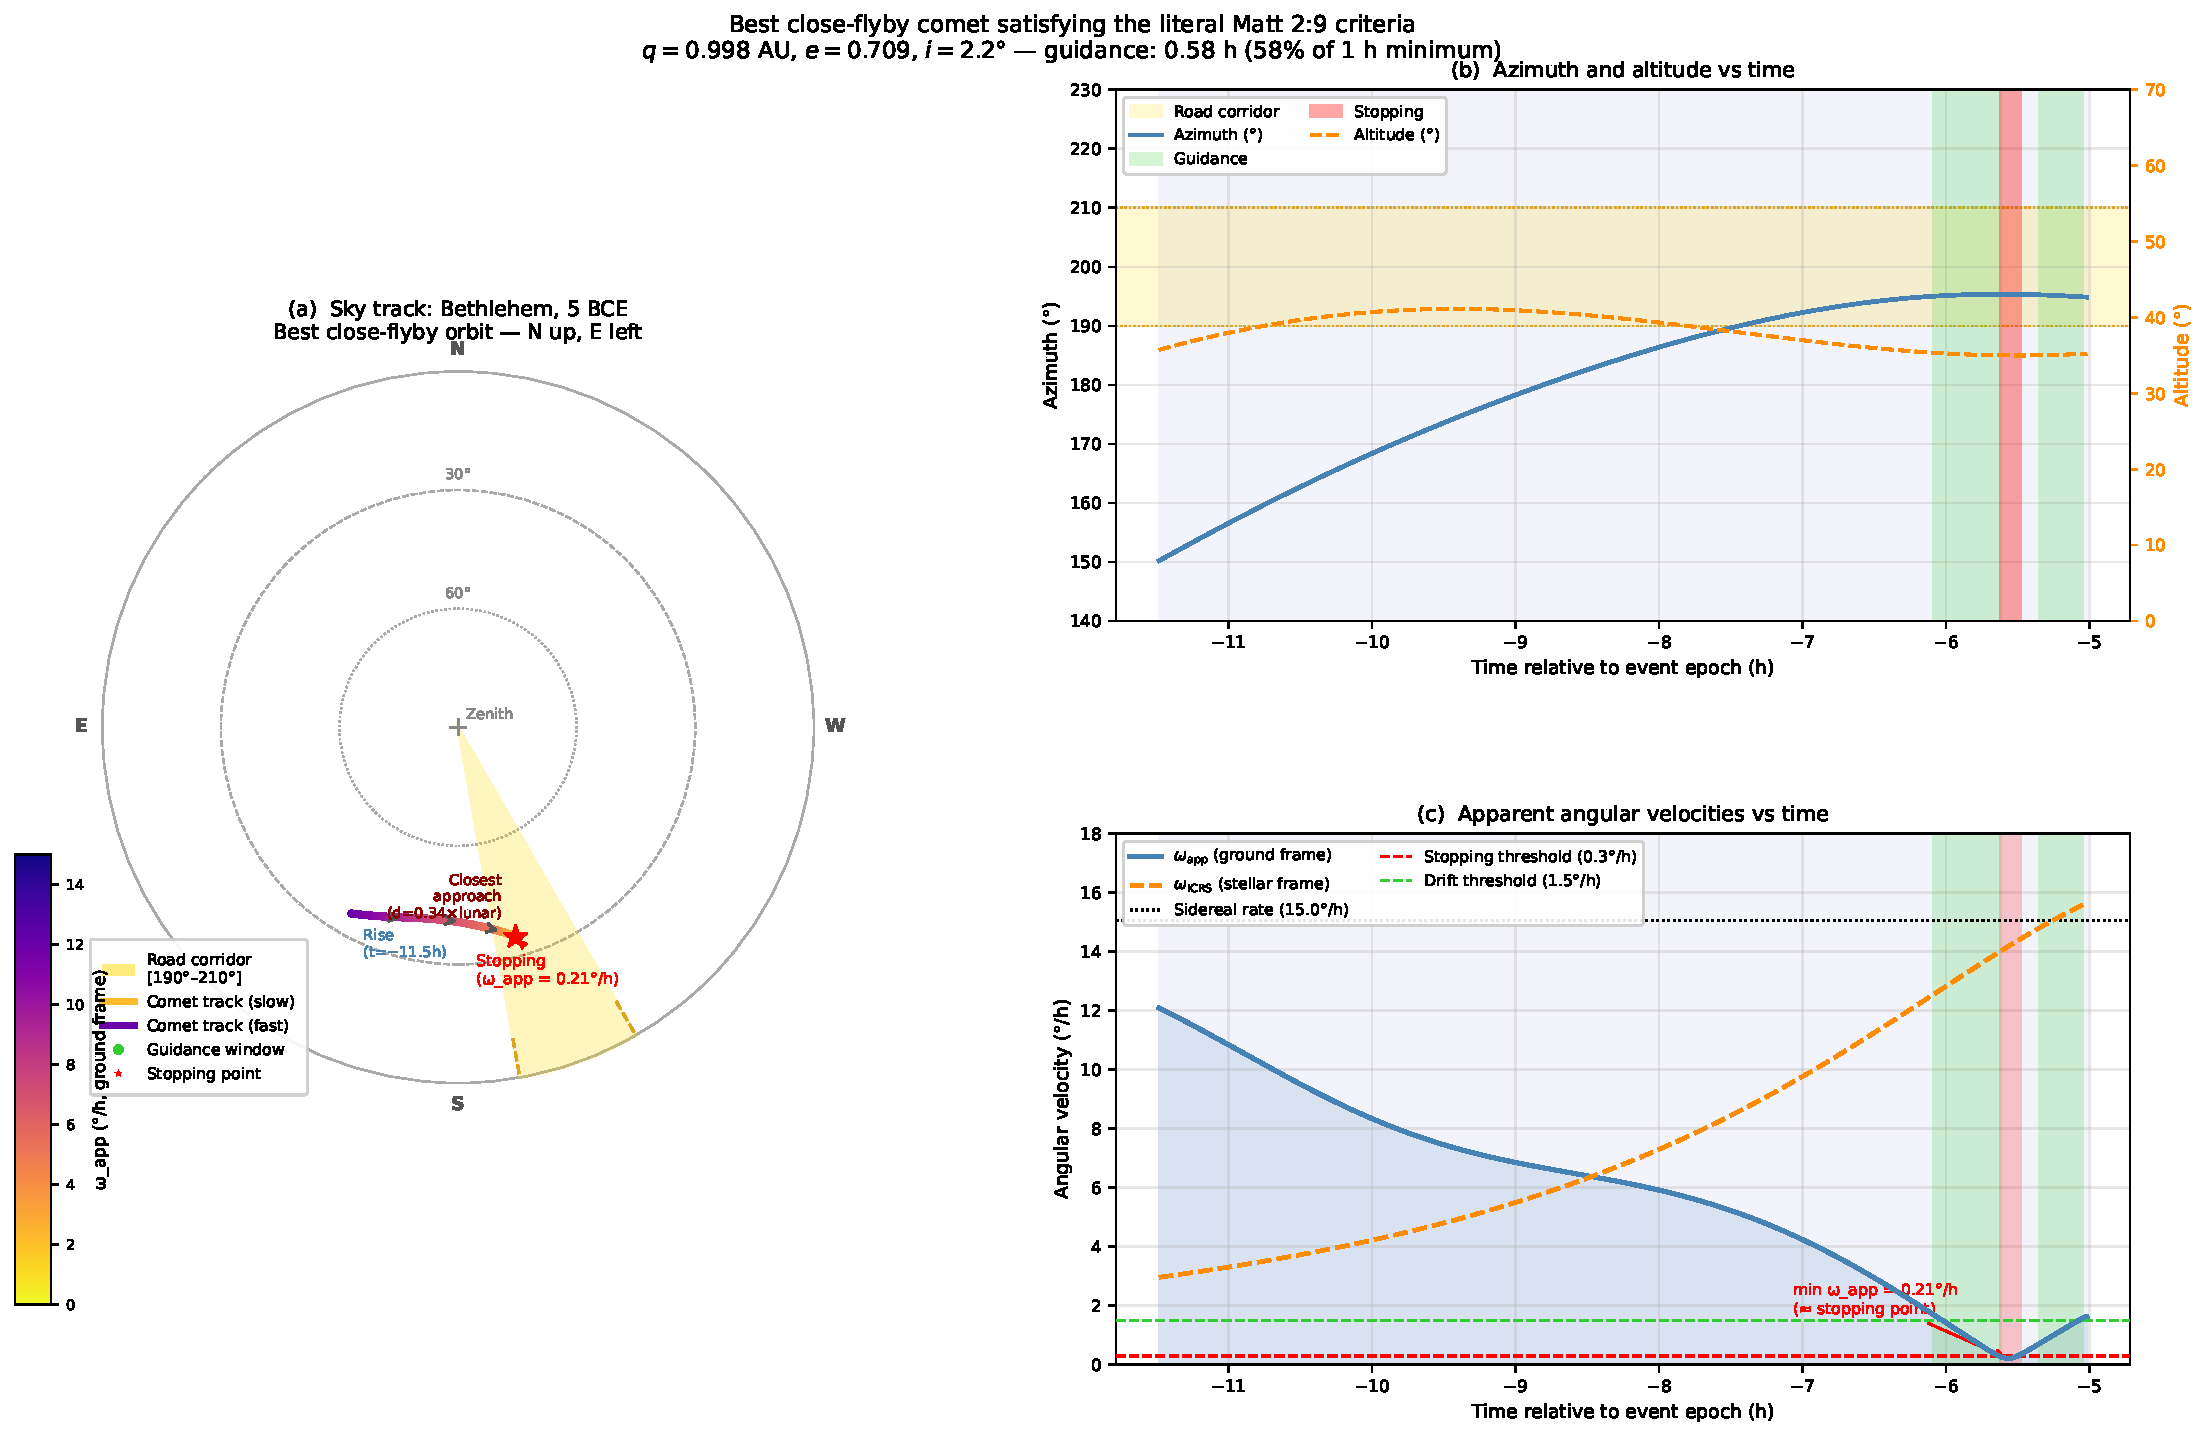
\includegraphics[width=\linewidth]{figure_flyby_bestorbit}
  \caption{%
    \textbf{Best close-flyby orbit satisfying the literal Matt~2:9 criteria.}
    \textbf{(a)}~Stereographic sky chart (N\,up, E\,left) as seen from Bethlehem
    during the night of 5~BCE Jun~8. The comet track (colored by ground-frame
    apparent velocity $\omega_\mathrm{app}$; dark = slow, bright = fast) rises in
    the east-southeast and sweeps westward under diurnal motion. The gold wedge
    marks the road corridor $[190^\circ, 210^\circ]$; green dots mark the guidance
    windows ($\approx\!46$~min total in two segments); the red star marks the stopping
    point ($\omega_\mathrm{app,min} = 0.21^\circ\,\mathrm{h}^{-1}$, 8~min duration) at
    $d \approx 0.34$~lunar distances. The comet penetrates only $5^\circ$ into
    the corridor (reaching az\,$\approx 195^\circ$) and never reaches azimuth $200^\circ$.
    \textbf{(b)}~Azimuth and altitude vs.\ time: the comet remains east of the
    corridor ($\mathrm{az} < 190^\circ$, below the gold band) for the entire
    night except the final $\approx\!1$~h.
    \textbf{(c)}~Ground-frame apparent velocity $\omega_\mathrm{app}$ (solid blue)
    and ICRS proper motion $\omega_\mathrm{ICRS}$ (dashed orange) vs.\ time.
    The brief crossing of $\omega_\mathrm{ICRS} \approx \omega_\mathrm{sid}$
    (sidereal rate; black dotted) produces the short stopping window.
    Green shading = guidance windows; red shading = stopping window.}
  \label{fig:flyby_bestorbit}
\end{figure}

\bibliographystyle{sn-nature}
\bibliography{sob_refs}

\end{document}
